% Soubory musí být v kódování, které je nastaveno v příkazu \usepackage[...]{inputenc}

\documentclass[%        Základní nastavení
%  draft,    				  % Testovací překlad
  12pt,       				% Velikost základního písma je 12 bodů
  a4paper,    				% Formát papíru je A4
  %oneside,      			% Jednostranný tisk
	twoside,      			% Dvoustranný tisk (kapitoly a další důležité části tedy začínají na lichých stranách)
	unicode,						% Záložky a metainformace ve výsledném  PDF budou v kódování unicode
]{report}				    	% Dokument třídy 'zpráva', vhodná pro sazbu závěrečných prací s kapitolami

\usepackage[utf8]		  %	Kódování zdrojových souborů je UTF-8
	{inputenc}					% Balíček pro nastavení kódování zdrojových souborů

\usepackage[				  % Nastavení geometrie stránky
	bindingoffset=10mm,		% Hřbet pro vazbu
	hmargin={25mm,25mm},	% Vnitřní a vnější okraj  (jsou nehezky shodné; jakási úroveň estetiky je dosažena pomocí hřbetu)
	vmargin={25mm,34mm},	% Horní a dolní okraj
	footskip=17mm,			  % Velikost zápatí
	nohead,					      % Bez záhlaví
	marginparsep=2mm,		  % Vzdálenost marginálií
	marginparwidth=18mm,	% Šířka marginálií
]{geometry}

\usepackage{sectsty}
	%přetypuje nadpisy všech úrovní na bezpatkové, kromě \chapter, která je přenastavena zvlášť v thesis.sty
	\allsectionsfont{\sffamily}

\usepackage{graphicx} % Balíček 'graphicx' pro vkládání obrázků
											% Nutné pro vložení logotypů školy a fakulty

\usepackage{pgfplots} % grafýky
\usepackage{amssymb}

\usepackage[          % Balíček 'acronym' pro sazby zkratek a symbolů
	nohyperlinks				% Nebudou tvořeny hypertextové odkazy do seznamu zkratek
]{acronym}						
											% Nutné pro použití prostředí 'acronym' balíčku 'thesis'

\usepackage[
	breaklinks=true,		% Hypertextové odkazy mohou obsahovat zalomení řádku
	hypertexnames=false, % Názvy hypertext. odkazů budou tvořeny nezávisle na názvech TeXu
  % colorlinks=false,    % Bez barevných odkazů
  hidelinks            % Bez rámečků kolem odkazů
]{hyperref}						% Balíček 'hyperref' pro sazbu hypertextových odkazů
											% Nutné pro použití příkazu 'pdfsettings' balíčku 'thesis'

\usepackage{pdfpages} % Balíček umožňující vkládat stránky z PDF souborů
                      % Nutné při vkládání titulních listů a zadání přímo
                      % ve formátu PDF z informačního systému

\usepackage{enumitem} % Balíček pro nastavení mezerování v odrážkách
  \setlist{topsep=0pt,partopsep=0pt,noitemsep} % konkrétní nastavení

\usepackage{cmap} 		% Balíček cmap zajišťuje, že PDF vytvořené `pdflatexem' je
											% plně "prohledávatelné" a "kopírovatelné"

%\usepackage{upgreek}	% Balíček pro sazbu stojatých řeckých písmem
											%% např. stojaté pí: \uppi
											%% např. stojaté mí: \upmu (použitelné třeba v mikrometrech)
											%% pozor, grafická nekompatibilita s fonty typu Computer Modern!
                      
%\usepackage{amsmath} %balíček pro sabu náročnější matematiky                 

\usepackage{dirtree}	% sazba adresářové struktury
                      % vhodné pro prezentaci obsahu elektronické přílohy (např. CD)

%====== Bibtex =====

\usepackage{csquotes}
\usepackage[style=iso-numeric]{biblatex}
\addbibresource{text/literatura.bib}



\usepackage[formats]{listings}	% Balíček pro sazbu zdrojových textů
\lstset{              % nastavení
%	Definice jazyka použitého ve výpisech
%    language=[LaTeX]{TeX},	% LaTeX
%	language={Matlab},		% Matlab
	language={C},           % jazyk C
    basicstyle=\ttfamily,	% definice základního stylu písma
    tabsize=2,			% definice velikosti tabulátoru
    inputencoding=utf8,         % pro soubory uložené v kódování UTF-8
		columns=fixed,  %fixed nebo flexible,
		fontadjust=true %licovani sloupcu
    extendedchars=true,
    literate=%  definice symbolů s diakritikou
    {á}{{\'a}}1
    {č}{{\v{c}}}1
    {ď}{{\v{d}}}1
    {é}{{\'e}}1
    {ě}{{\v{e}}}1
    {í}{{\'i}}1 
    {ó}{{\'o}}1
    {ř}{{\v{r}}}1
    {š}{{\v{s}}}1
    {ť}{{\v{t}}}1
    {ú}{{\'u}}1
    {ů}{{\r{u}}}1
    {ý}{{\'y}}1
    {ž}{{\v{z}}}1
    {Á}{{\'A}}1
    {Č}{{\v{C}}}1
    {Ď}{{\v{D}}}1
    {É}{{\'E}}1
    {Ě}{{\v{E}}}1
    {Í}{{\'I}}1
    {Ň}{{\v{N}}}1
    {Ó}{{\'O}}1
    {Ř}{{\v{R}}}1
    {Š}{{\v{S}}}1
    {Ť}{{\v{T}}}1
    {Ú}{{\'U}}1
    {Ů}{{\r{U}}}1
    {Ý}{{\'Y}}1
    {Ž}{{\v{Z}}}1
}

%%%%%%%%%%%%%%%%%%%%%%%%%%%%%%%%%%%%%%%%%%%%%%%%%%%%%%%%%%%%%%%%%
%%%%%%      Definice informací o dokumentu             %%%%%%%%%%
%%%%%%%%%%%%%%%%%%%%%%%%%%%%%%%%%%%%%%%%%%%%%%%%%%%%%%%%%%%%%%%%%

% V tomto souboru se nastavují téměř veškeré informace, proměnné mezi studenty:
% jméno, název práce, pohlaví atd.
% Tento soubor je SDÍLENÝ mezi textem práce a prezentací k obhajobě -- netřeba něco nastavovat na dvou místech.

\usepackage[
%%% Z následujících voleb jazyka lze použít pouze jednu
  czech-english,		% originální jazyk je čeština, překlad je anglicky (výchozí)
  %english-czech,	  % originální jazyk je angličtina, překlad je česky
  %slovak-english,	% originální jazyk je slovenština, překlad je anglicky
  %english-slovak,	% originální jazyk je angličtina, překlad je slovensky
%
%%% Z následujících voleb typu práce lze použít pouze jednu
  semestral,		  % semestrální práce (výchozí)
  %bachelor,			%	bakalářská práce
  %master,			  % diplomová práce
  %treatise,			% pojednání o disertační práci
  %doctoral,			% disertační práce
%
%%% Z následujících voleb zarovnání objektů lze použít pouze jednu
%  left,				  % rovnice a popisky plovoucích objektů budou zarovnány vlevo
	center,			    % rovnice a popisky plovoucích objektů budou zarovnány na střed (vychozi)
%
]{thesis}   % Balíček pro sazbu studentských prací


%%% Jméno a příjmení autora ve tvaru
%  [tituly před jménem]{Křestní}{Příjmení}[tituly za jménem]
% Pokud osoba nemá titul před/za jménem, smažte celý řetězec '[...]'
\author[]{Tomáš}{Vavrinec}

%%% Identifikační číslo autora (VUT ID)
\butid{240893}

%%% Pohlaví autora/autorky
% (nepoužije se ve variantě english-czech ani english-slovak)
% Číselná hodnota: 1...žena, 0...muž
\gender{0}

%%% Jméno a příjmení vedoucího/školitele včetně titulů
%  [tituly před jménem]{Křestní}{Příjmení}[tituly za jménem]
% Pokud osoba nemá titul před/za jménem, smažte celý řetězec '[...]'
\advisor[doc.\ Ing..]{Pavel}{Šteffan}[Ph.D.]

%%% Jméno a příjmení oponenta včetně titulů
%  [tituly před jménem]{Křestní}{Příjmení}[tituly za jménem]
% Pokud osoba nemá titul před/za jménem, smažte celý řetězec '[...]'
% Nastavení oponenta se uplatní pouze v prezentaci k obhajobě;
% v případě, že nechcete, aby se na titulním snímku prezentace zobrazoval oponent, pouze příkaz zakomentujte;
% u obhajoby semestrální práce se oponent nezobrazuje (jelikož neexistuje)
% U dizertační práce jsou typicky dva až tři oponenti. Pokud je chcete mít na titulním slajdu, prosím ručně odkomentujte a upravte jejich jména v definici "VUT title page" v souboru thesis.sty.
\opponent[doc.\ Mgr.]{Křestní}{Příjmení}[Ph.D.]

%%% Název práce
%  Parametr ve složených závorkách {} je název v originálním jazyce,
%  parametr v hranatých závorkách [] je překlad (podle toho jaký je originální jazyk).
%  V případě, že název Vaší práce je dlouhý a nevleze se celý do zápatí prezentace, použijte příkaz
%  \def\insertshorttitle{Zkác.\ náz.\ práce}
%  kde jako parametr vyplníte zkrácený název. Pokud nechcete zkracovat název, budete muset předefinovat,
%  jak se vytváří patička slidu. Viz odkaz: https://bit.ly/3EJTp5A
\title[Title of Student's Thesis]{Automatické herní stanoviště}

%%% Označení oboru studia
%  Parametr ve složených závorkách {} je název oboru v originálním jazyce,
%  parametr v hranatých závorkách [] je překlad
\specialization[Microelectronics and Technology]{Mikroelektronika a technologie}

%%% Označení ústavu
%  Parametr ve složených závorkách {} je název ústavu v originálním jazyce,
%  parametr v hranatých závorkách [] je překlad
%\department[Department of Control and Instrumentation]{Ústav automatizace a měřicí techniky}
%\department[Department of Biomedical Engineering]{Ústav biomedicínského inženýrství}
%\department[Department of Electrical Power Engineering]{Ústav elektroenergetiky}
%\department[Department of Electrical and Electronic Technology]{Ústav elektrotechnologie}
%\department[Department of Physics]{Ústav fyziky}
%\department[Department of Foreign Languages]{Ústav jazyků}
%\department[Department of Mathematics]{Ústav matematiky}
\department[Department of Microelectronics]{Ústav mikroelektroniky}
%\department[Department of Radio Electronics]{Ústav radioelektroniky}
%\department[Department of Theoretical and Experimental Electrical Engineering]{Ústav teoretické a experimentální elektrotechniky}
% \department[Department of Telecommunications]{Ústav telekomunikací}
%\department[Department of Power Electrical and Electronic Engineering]{Ústav výkonové elektrotechniky a elektroniky}

%%% Označení fakulty
%  Parametr ve složených závorkách {} je název fakulty v originálním jazyce,
%  parametr v hranatých závorkách [] je překlad
%\faculty[Faculty of Architecture]{Fakulta architektury}
\faculty[Faculty of Electrical Engineering and~Communication]{Fakulta elektrotechniky a~komunikačních technologií}
%\faculty[Faculty of Chemistry]{Fakulta chemická}
%\faculty[Faculty of Information Technology]{Fakulta informačních technologií}
%\faculty[Faculty of Business and Management]{Fakulta podnikatelská}
%\faculty[Faculty of Civil Engineering]{Fakulta stavební}
%\faculty[Faculty of Mechanical Engineering]{Fakulta strojního inženýrství}
%\faculty[Faculty of Fine Arts]{Fakulta výtvarných umění}
%
%Nastavení logotypu (v hranatych zavorkach zkracene logo, ve slozenych plne):
\facultylogo[logo/FEKT_zkratka_barevne_PANTONE_CZ]{logo/UTKO_color_PANTONE_CZ}

%%% Rok odevzdání práce
\graduateyear{2023}
%%% Akademický rok odevzdání práce
\academicyear{2023/24}

%%% Datum obhajoby (uplatní se pouze v prezentaci k obhajobě)
\date{11.\,11.\,1980} 

%%% Místo obhajoby
% Na titulních stránkách bude automaticky vysázeno VELKÝMI písmeny (pokud tyto stránky sází šablona)
\city{Brno}

%%% Abstrakt
\abstract[%
The aim of this thesis is to design an electronic device for use in outdoor games. 
Primarily the design of an automatic gaming station, but there has also been a design of a simple personal device. 
This thesis deals with the selection and rough design of the electronics.
Emphasis is placed on the selection of appropriate systems for application in games and the design of electronics based on these.
The design is divided into several groupings, the personal device design and the game station design which is further divided into the design of the core and its modules.
]{%
Cílem práce je navrhnout elektronické zařízení pro využití v outdorových hrách. 
Primárně jde o návrh automatického herního stanoviště, ale došlo i k návrhu jednoduchého osobního zařízení. 
Tato práce se zabývá teoretickým návrhem elektroniky.
Je kladen důraz na výběr vhodných systémů k aplikaci ve hrách a z nich vychází návrh elektroniky.
Návrh je rozdělen do několika skupin, návrh osobního zařízení a návrh herního stanoviště, který se dále dělí na návrh jádra a jeho modulů.
}

%%% Klíčová slova
\keywrds[%
microcontroller, ESP32, ESP32-C3-MINI-1, ESP32-S3, ESP32-S3-WROOM, outdoor games, gaming stations, gaming facilities
]{%
mikrokontrolér, ESP32, ESP32-C3-MINI-1, ESP32-S3, ESP32-S3-WROOM, outdoorové hry, herní stanoviště, herní zařízení
% Klíčová slova v~originálním jazyce
}

%%% Poděkování
\acknowledgement{%
Rád bych poděkoval vedoucímu semestrální práce
panu doc. Ing. Pavlu Šteffanovi, Ph.D.\ za odborné vedení,
konzultace, trpělivost a~podnětné návrhy k~práci.
}%  % do tohoto souboru doplňte údaje o sobě, druhu práce, názvu...

%%%%%%%%%%%%%%%%%%%%%%%%%%%%%%%%%%%%%%%%%%%%%%%%%%%%%%%%%%%%%%%%%%%%%%%%

%%%%%%%%%%%%%%%%%%%%%%%%%%%%%%%%%%%%%%%%%%%%%%%%%%%%%%%%%%%%%%%%%%%%%%%%
%%%%%%     Nastavení polí ve Vlastnostech dokumentu PDF      %%%%%%%%%%%
%%%%%%%%%%%%%%%%%%%%%%%%%%%%%%%%%%%%%%%%%%%%%%%%%%%%%%%%%%%%%%%%%%%%%%%%
%% Při načteném balíčku 'hyperref' lze použít příkaz '\pdfsettings':
\pdfsettings
%  Nastavení polí je možné provést také ručně příkazem:
%\hypersetup{
%  pdftitle={Název studentské práce},    	% Pole 'Document Title'
%  pdfauthor={Autor studenstké práce},   	% Pole 'Author'
%  pdfsubject={Typ práce}, 						  	% Pole 'Subject'
%  pdfkeywords={Klíčová slova}           	% Pole 'Keywords'
%}
%%%%%%%%%%%%%%%%%%%%%%%%%%%%%%%%%%%%%%%%%%%%%%%%%%%%%%%%%%%%%%%%%%%%%%%

\pdfmapfile{=vafle.map}

%%%%%%%%%%%%%%%%%%%%%%%%%%%%%%%%%%%%%%%%%%%%%%%%%%%%%%%%%%%%%%%%%%%%%%%
%%%%%%%%%%%       Začátek dokumentu               %%%%%%%%%%%%%%%%%%%%%
%%%%%%%%%%%%%%%%%%%%%%%%%%%%%%%%%%%%%%%%%%%%%%%%%%%%%%%%%%%%%%%%%%%%%%%
\begin{document}
\pagestyle{empty} %vypnutí číslování stránek

%%% Vložení desek -- od září 2021 na žádost fakulty nepoužíváno
%\includepdf[pages=1]%  buďto generovaných informačním systémem
  %{pdf/student-desky}% název souboru nesmí obsahovat mezery!
%%% NEBO vytvoření desek z balíčku
%%\makecover
%%%
%\oddpage % při dvojstranném tisku přidá prázdnou stránku
%% kazdopádně ale:
%\setcounter{page}{1} %resetovaní čítače stránek -- desky do číslování nezahrnujeme

%% Vložení titulního listu
\includepdf[pages=1]%    buďto generovaného informačním systémem
  {pdf/student-titulka}% název souboru nesmí obsahovat mezery!
%% NEBO vytvoření titulní stránky z balíčku
%\maketitle
%%
\oddpage  % při dvojstranném tisku se přidá prázdná stránka
   
%% Vložení zadání
\includepdf[pages=1]%   buďto generovaného informačním systémem
  {pdf/student-zadani}% název souboru nesmí obsahovat mezery!
%% NEBO lze vytvořit prázdný list příkazem ze šablony
%\patternpage{}%
%	{\sffamily\Huge\centering ZDE VLOŽIT LIST ZADÁNÍ}%
%	{\sffamily\centering Z~důvodu správného číslování stránek}
%%
\oddpage  % při dvojstranném tisku se přidá prázdná stránka

%% Vysázení stránky s abstraktem
\makeabstract

%%% Vysázení citace práce
\makecitation

%%% Vysázení prohlášení o samostatnosti
\makedeclaration

%%% Vysázení poděkování
\makeacknowledgement

%%% Vysázení obsahu
\tableofcontents

%%% Vysázení seznamu obrázků
% (vynechejte, pokud máte dva nebo méně obrázků)
\listoffigures

% %%% Vysázení seznamu tabulek
% % (vynechejte, pokud máte dvě nebo méně tabulek)
% \listoftables

% %%% Vysázení seznamu výpisů kódu
% % (vynechejte, pokud máte dva nebo méně výpisů)
% \lstlistoflistings

\cleardoublepage\pagestyle{plain}   % zapnutí číslování stránek

%Pro vkládání kapitol i příloh používejte raději \include než \input
%%% Vložení souboru 'text/uvod.tex' s úvodem

\chapter*{Úvod}
%Automatické herní stanoviště (AHS) je nástroj pro tvorbu outdoorových her.
Outdoorové hry bývají často složeny ze stanovišť, na kterých mají hráči plnit různé úkoly.
Aby bylo možné tyto úkoly zadat a vyhodnotit jejich výsledek, je většinou nutné, aby na stanovišti byl nějaký organizátor a stanoviště obsluhoval.
Tyto úkoly jsou ale často poměrně prosté a není tak problém je automatizovat, což může organizátory uvolnit k jiné činnosti.
Outdoorové hry by navíc znatelně oživila aktivní komunikace mezi stanovištěmi, která by tak mohla i vytvořit prostor pro nové herní mechaniky.

Řada outdoorových her využívá různé podomácku vyrobené zařízení, které nějaký z organizátorů postavil za účelem konkrétní hry.
Taková zařízení ale autora stojí velké množství času, protože jej musí celé od základu navrhnout, vyrobit a navíc je jej pak schopen obsluhovat jen on.
Navíc je pak takové zařízení typicky použito jen u jedné nebo dvou her, po kterých jej autor buď, rozebere, nebo bezpečně uloží někam, kde si jej náhodou všimne o deset let později při úklidu.
V neposlední řadě bývají jakýmsi zlatým hřebem celé akce např. týdenního tábora a jejich kouzlo je především v odlišnosti od zbytku akce.



Z těchto důvodů padlo rozhodnutí na vývoj univerzálního automatického herního stanoviště, které by se dalo opakovaně použít na různé hry i ve větší počtu.
Podstatnou součástí je pochopitelně i pokud možno co nejintuitivnější ovládání, aby uživatele nezdržovalo od zábavy.


% % Úvod studentské práce, např\,\dots

% % Nečíslovaná kapitola Úvod obsahuje \uv{seznámení} čtenáře s~problematikou práce.
% % Typicky se zde uvádí:
% % (a) do jaké tematické oblasti práce spadá, (b) co jsou hlavní cíle celé práce a (c) jakým způsobem jich bylo dosaženo.
% % Úvod zpravidla nepřesahuje jednu stranu.
% % Poslední odstavec Úvodu standardně představuje základní strukturu celého dokumentu.

% % Tato práce se věnuje oblasti \acs{DSP} (\acl{DSP}), zejména jevům, které nastanou při nedodržení Nyquistovy podmínky pro \ac{symfvz}.%
% % \footnote{Tato věta je pouze ukázkou použití příkazů pro sazbu zkratek.}

% % Šablona je nastavena na \emph{dvoustranný tisk}.
% % Nebuďte překvapeni, že ve vzniklém PDF jsou volné stránky.
% % Je to proto, aby důležité stránky jako např.\ začátky kapitol začínaly po vytisknutí a svázání vždy na pravé straně.
% % %
% % Pokud máte nějaký závažný důvod sázet (a~zejména tisknout) jednostranně, nezapomeňte si přepnout volbu \texttt{twoside} na \texttt{oneside}!

% %%% Vložení souboru 'text/cile.tex' s úvodem
% \chapter*{Cíle práce}
\phantomsection
\addcontentsline{toc}{chapter}{Cíle práce}

Konkrétní specifikace cílů, které má autor v~práci vyřešit.
Tato kapitola je \emph{volitelná} -- pokud váš studijní program nevyžaduje zvláštní kapitolu s cíli,
cíle specifikujte v~rámci Úvodu.

%%% Vložení souboru 'text/reseni' s popisem řešení práce
% (rozdělte na více souborů či kapitol, pokud je vhodné)
\chapter{Důvody elektronizace zážitkových her}
% \chapter{Motivace pro elektronizaci zážitkové pedagogiky}
Outdoorové hry často mají nějaký příběh, který se dá vyprávět konkrétními úkoly na stanovištích.
Na některých stanovištích proto musí být lidská obsluha, na jiných ale může být lidská obsluha z příběhového pohledu nežádoucí.
Když má hráč například vyřadit automatický bezpečnostní systém je lidská obsluha stanoviště poslední možnost.
Podobná stanoviště proto bývají realizovány pomocí různých papírků a provázků.
To určitě má své kouzlo, ale i tak je u podobného stanoviště vhodné mít obsluhu.
Elektronické řešení podobných stanovišť by ale mohlo otevřít úplně nový svět možností.

%% Položme si tedy otázku, jak by takové zařízení mohlo vypadat.
Podstatný fakt je, že prakticky všichni u sebe dnes mají chytrý telefon, čehož můžeme využít.
Nemá proto velký význam, aby toto zařízení suplovalo funkce telefonu.
Např. grafický výstup typu display proto v podobném zařízení není potřeba, a v tomto směru už odvádí telefon naprosto dostatečnou práci.
Pokud by tedy v rámci hry bylo potřeba například předat hráči nějaký text nebo obrázek, může jej zařízení poslat uživateli na telefon.
Možnost propojení s telefonem je také velmi významná při nastavování hry.
Díky telefonu totiž zařízení nepotřebuje uživatelské rozhraní přizpůsobené nastavování.

Mohlo by se zdát, že herní stanoviště vlastně ani není potřeba a stačila by mobilní aplikace.
Ale přestože je mobil ve hrách dobře využitelný, jsou aplikace, na které jednoduše vhodný není.
Pokud má hráč například ze stanoviště získat nějaký fyzický objekt, mobil neposlouží.
Pro hráče ani organizátory také nemusí být zrovna komfortní před hrou zařizovat, aby měli všichni nainstalovaný správný software.
% Telefon také není například na stanovišti v lese dobře viditelný.
V neposlední řadě jde také o jistý "cool efekt", který běžné zařízení jako mobil nebo třeba tablet neposkytne. %%TODO: tohle chce nějak přeformulovat

Zařízení určené primárně pro outdoorové hry bychom mohli rozdělit na dvě skupiny, statické a dynamické, protože jsou na tyto skupiny kladeny výrazně jiné požadavky.
Dynamická zařízení jsou ta, která může uživatel pohodlně nosit s sebou.
Do dynamických zařízení by se tak dal zařadit právě i telefon, ten však může být z různých důvodu nevhodný a proto i tato zařízení dává smysl navrhnout specificky pro hry.
Statické zařízení je naopak zařízení, u kterého se nepředpokládá, že jej bude hráč nosit s sebou.
Přesto by mělo být jednoduše přenositelné, má jít o stanoviště, které se jednoduše donese na své místo a během hry se s ním nebude pohybovat.
Takové zařízení by tedy mělo být dobře viditelné a splňovat požadavky, které na něj konkrétní hra klade. %%TODO: tohle chce nějak přeformulovat?
Požadavky různých her můžou být ale dost rozdílné, častým požadavkem je něco uchovávat a např. po zadání hesla hráči vydat.
Hra ale taky může vyžadovat, aby bylo zařízení sto přehrát nějakou audio nahrávku nebo naopak pořídit záznam. %%TODO: tohle chce nějak přeformulovat?
Z těchto důvodů považujeme za vhodnější zařízení koncipovat jako základní řídící jednotku, která je samostatně funkční a použitelná při hře, ale ke které se dají jednoduše připojit moduly pro konkrétní herní mechaniky.

\section{Základní řídící jednotka}
% Z toho plyne otázka, jaká funkcionalita je potřebná v základním zařízení?
Asi žádný systém, se kterým hráč přímo interaguje, není nutný v každé hře.
Jde tedy o to vybrat takové systémy, které svými nároky nepřevýší užitečnost při hrách.
Ze zkušeností považujeme za nejzákladnější systém nějaký světelný výstup, ten dokáže většinu her velmi příjemně ozvláštnit.
Většinou je nezbytný i nějaký uživatelský vstup, na což většinou stačí obyčejná tlačítka.
Problém je ale určit jaké a kolik jich bude potřeba.
Některé hry vyžadují třeba jen jedno, ale takové, aby se do něj dalo co nejpohodlněji praštit v běhu, protože je zrovna cílem ke stanovišti co nejrychleji doběhnout.
Jiná hra může vyžadovat tlačítek víc, ale už není potřeba, aby byly tak velké, protože hráč při jejich používání nebude tak akční, ale bude třeba zadávat výsledek nějakého logického úkolu.
Univerzálnější je tedy nepoužívat tlačítka, ale nějaký systém, který se dá softwarově přizpůsobit.
Příkladem může být dotyková plocha, která se dá softwarově rozdělit na různé oblasti sloužící jako tlačítka a i během hry se tak dá počet tlačítek měnit.
Další důležitou vlastností je možnost komunikace s ostatními zařízeními, která do hry přináší novou možnost jak stanoviště propojit a také pohodlnou metodu jak stanoviště nastavit přes telefon.
V neposlední řade je potřeba nějaký zvukový výstup, který může být použit např. jako potvrzení zadaného hesla.

Z toho nám tedy plyne diagram \ref{fig:diagram_zanoreni_0}.
\begin{figure}[h]
    \centering
    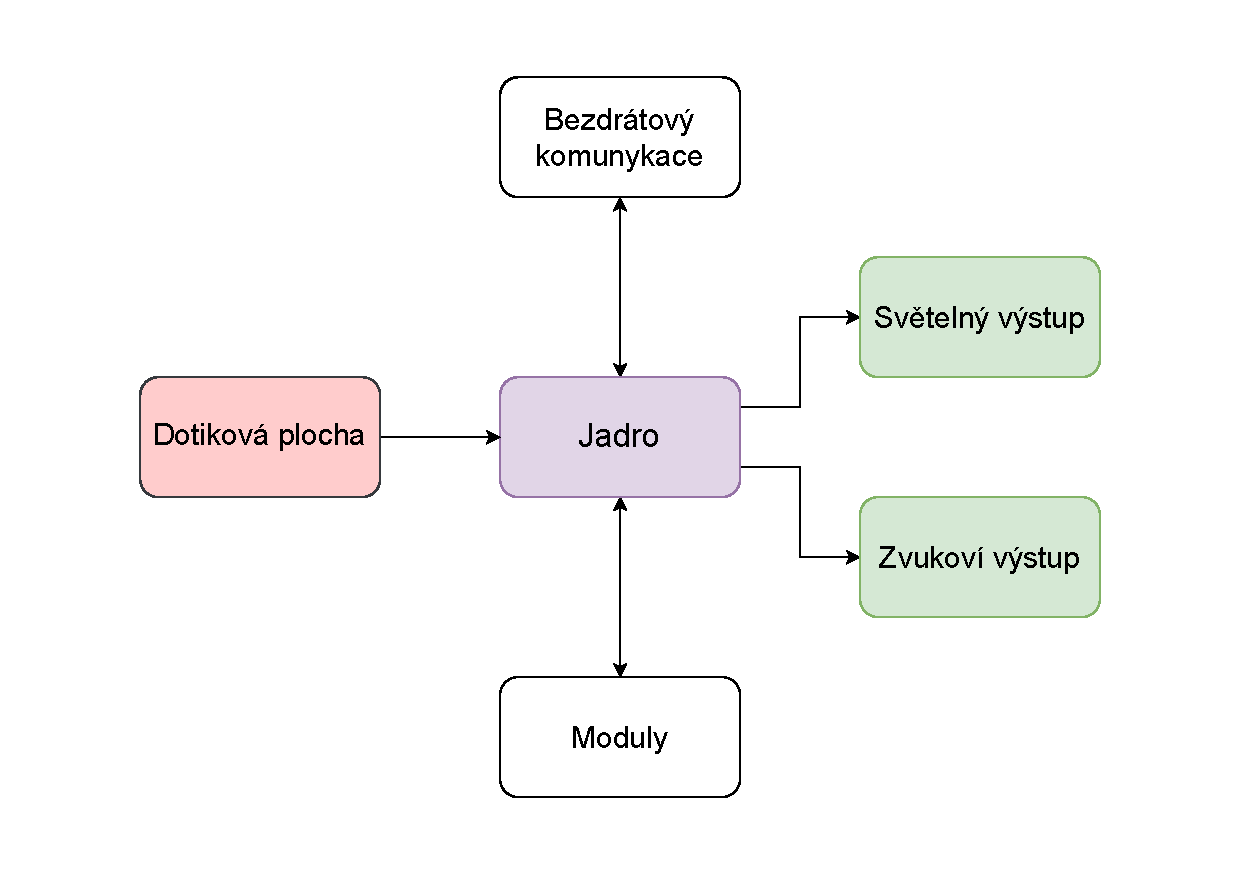
\includegraphics[width=0.65\textwidth]{text/TeoretickyUvod/AplikaceHernichZarizeni/diagram/zanoreni_0.pdf}
    \caption{Úvodní blokové schéma zařízení}
    \label{fig:diagram_zanoreni_0}
\end{figure}

\newpage

Co se světelného výstupu týče, na signalizaci různých stavů je vhodné používat různé barvy světel.
% Jaký vzhled by ale měl mít zdroj barevného světla na podobném zařízení?
Jak je uvedeno výše, není potřebné suplovat grafický display, za tímto účelem se dá použít propojení s telefonem.
Informace, kterou by zařízením mohlo často poskytovat je čas a směr, např. čas do konce kola nebo směr k dalšímu úkolu.
Podobné informace se dají elegantně zobrazit na kruhu.
Protože má být stanoviště viditelné i z větší vzdálenosti, je tedy otázkou, zda použít jen jeden kruh, tak aby byl dostatečně viditelný, nebo jich použít více. %%TODO: otázka co s totu otázkou?
Zobrazování pracuje ve dvou režimech, čtení na dálku a čtení na blízko.
Pro čtení na blízko je cílem přímá interakce se zařízením např. už zmiňované zadávání hesla.
Čtení na dálku je naopak určeno pro předávání informací hráči, když právě přímo neinteraguje se stanovištěm, např. který tým má zrovna povolený přístup.
Proto je vhodné mít kruhů víz, aby bylo možné zobrazovat tyto informace na různých kruzích, které mohou navíc být svému účelu přizpůsobeny.
Jeden kruh tak může svítit jen jedním směrem aby ho hráč vyděl celí najednou pro blízkou interakci, zatímco druhý kruh může svítit do všech stran aby byl vidět z co nejvíce míst.

Potřeba propojení s telefonem nám omezuje možnosti co se týče bezdrátové komunikace, protože telefony jsou většinou vybavený Bluetooth a WiFi.
Také se v telefonech rozšiřuje NFC, to je však pro tuto aplikaci z duvodu krátkého dosahu nevhodné.

Posledním systémem který je potřeba je zvukový výstup.
Protože většinou stačí jen jednoduchá zvuková odezva, není potřeba plnohodnotný zvukový systém.
Pro hry, které budou potřebovat přehrávat nějakou nahrávku bude samostatný zvukový modul, případně je možnost nahrávku přehrát přes uživatelův telefon.
V základním zařízení je proto potřeba jen jednoduchý bzučák, například jako odezva na kliknutí.

Můžeme tedy diagram upravit na \ref{fig:diagram_zanoreni_1}.
\begin{figure}[h]
    \centering
    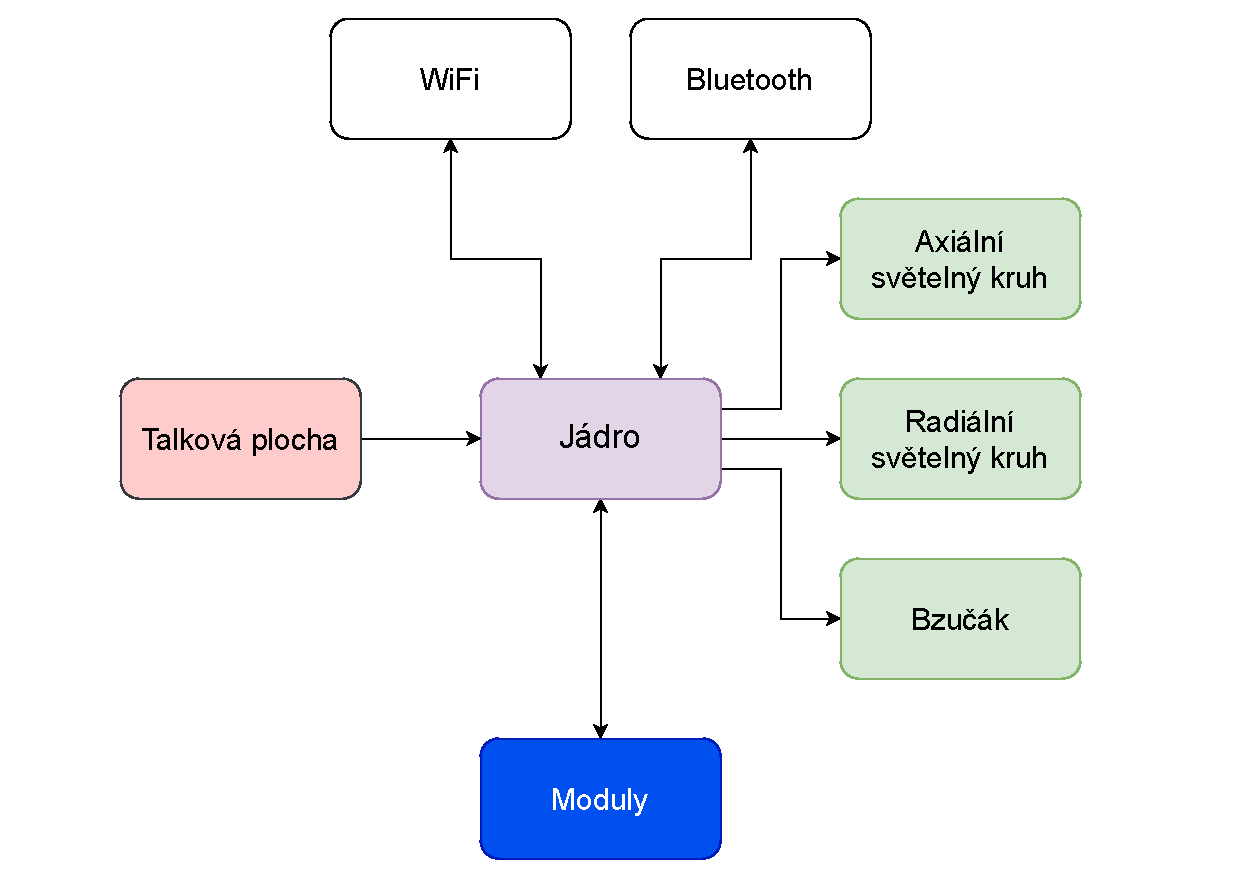
\includegraphics[width=0.65\textwidth]{text/TeoretickyUvod/AplikaceHernichZarizeni/diagram/zanoreni_1.pdf}
    \caption{Základního blokové schéma zařízení}
    \label{fig:diagram_zanoreni_1}
\end{figure}

\vspace{-10mm}
\section{Moduly}
Základní řídící jednotka je tedy schopná poskytnout základní funkce, které jsou potřeba pro většinu her.
Některé hry ale mohou vyžadovat nějakou specifickou funkci, kterou základní zařízení nedokáže poskytnout.
Proto je vhodné, aby bylo možné k základnímu zařízení připojit externí moduly, bez kterých by se konkrétní hry neobešli.

Jedním z takových modulů může být například modul dvířka, který umožní do zařízení uložit nějaký objekt a vydat jej jen po nějaké interakci.
Konkrétně má takový modul několik samostatných zamykatelných přihrádek, které se dají samostatně ovládat a mohou sloužit např. pro více týmů nebo uchovávat více objektu do různých částí hry.

Jednoduchá hrou která vyžaduje modul dvířka je např. hra Maják. %%TODO: vymyslet lepčí název tohle se  mi moc nepozdává (je to název z her od Petra na první lucerný v roce 2021)
V této hře jsou hráči rozděleni do týmů a každý tým má svou barvu, od které je odvozena konkrétní přihrádka. 
Týmy mají za úkol získat co nejvíc sad kartiček.
Na hřišti je několik automatických stanovišť s modulem dvířka a v každém z nich je nějaký typ kartičky.
Každé stanoviště během hry umožňuje přístup právě jednomu týmu, které v pravidelném intervalu mění a čas do změny reprezentuje na jednom z kruhů.
Při startu hry si každé stanoviště náhodně vybere tým kterým začne a následně se už drží konstantního pořadí.
Když někdo dorazí ke stanovišti ve chvíli kdy má stanoviště zpřístupnění jeho tým a klepne na tlakovou plochu, stanoviště mu vydá kartičku.
Stanoviště se týmu zpřístupní jen v čase daného týmu a navíc jen jednou za kolo.
Hráčům cíleně není představen celí mechanizmus výdeje kartiček, je jim řečeno jen že se přihrádka otevírá klepnutím do tlakové plochy a že je zajímají jen kartičky jejich barvi. 
Tým tedy musí spolupracovat nejprve na odhalení mechanizmu a následně myslet jak tedy zvítězit.

Podobná hra se duď dá hrát samostatně nebo muže jít například jen o metodu jak získávat suroviny v nějaké komplexnější hře.

Další modul, který se dá připojit je zvukový modul.
Hra který vyžaduje zvukový modul je například hra s názvem Ticho.
Tato hrá vyžaduje zároveň i modul dvířka.
V této hře stanoviště sleduje intenzitu zvuku v okoli a v momente kdy hluk klesne pod stanovenou úroveň stanoviště otevře dvířka. 
% Ucastnikum není ovládání představeno a musí tak na něj přijít samy.
Stanoviště je hráčům představeno jako "magicka krabicka" za carou ke ktere se nesmi proplížit ale muzou ji z dalky ovlivnit.
Ukolem hracu tak bylo prijit na to jak lucerna funguje a jak ji presvedci aby se otevřela.

V rámci zvukového modulu je i možnost přehrát nějakou nahrávku.
Tato část zvukového modulu umožňuje intenzivnější vtažení hráče do hry s příběhem.
Může jít například o unikovou hru při které hráč ocitne v oblasti v neznámém bludišti a jeho úkolem je najít cestu ven.
Při hledání muže narazit na různá stanoviště která mu nejprve přehrají nějakou část příběhu a následně mu dají nějaký úkol nebo radu jak postupovat dál.

Podstatným modulem je také komunikační modul který umožňuje připojení k mobilní síti a tím i komunikaci s ostatními zařízeními na velkou vzdálenost.
Tento modul je potřeba například pro hru Zábor kopce.

V této hře se na hřišti o velké rozloze nachází několik automatických stanovišť.
Hráči jsou rozděleni do týmů a každý tým má svou barvu a své tlačítko na stanovišti označené barvou týmu.
V hře Zábor Kopce je hlavním cílem získávat body pro svůj tým ovládnutím a udržením stanovišť na rozsáhlém hřišti. 
Axiálním světelný kruh zobrazuje rozdělení tlakové plochu na jednotlivá tlačítka týmů podle jejich barvi.
Zabrání stanoviště pak mohou hráči provést stiskem příslušného tlačítka. 
Získávání bodů se odehrává dvěma způsoby, ovládnutím stanoviště a následným držením stanoviště pod kontrolou. 
Týmy mohou přebírat stanoviště od soupeřů, což přidává hře strategický rozměr. 
Výhodou je kontrolovat více stanovišť najednou, což umožňuje rychlejší získávání bodů a zvyšuje šanci na vítězství.
Komunikační modul je tu potřebný pro vyhodnocování hry.
Stanoviště totiž musí být schopné komunikovat s centrálním serverem, který vyhodnocuje hru a zobrazuje její průběh.
Tato hra je původně navržena pro airsoftové hráče na hřiště v Mokra-Horakov o rozloze \(6.7\-[ha]\) \cite{MokraHorakov}.
V takovém prostředí je tedy komunikace pomocí WiFi či Bluetooth nedostačuje, protože stanoviště mohou být i několik set metrů od sebe.

\subsection{Výběr bezdrátové komunikace dlouhého dosahu}
Pro komunikaci na dlouhé vzdálenosti se nabízí asi jen dvě základní možnosti, LoRa a mobilní síť.
Ještě počátkem roku 2023 by byla i třetí možnost, Sigfox, ale jeho síť byla v ČR vypnuta \cite{SigfoxKonci}.

LoRa je technologie určená pro komunikaci na dlouhé vzdálenosti s malou spotřebou a datovou propustností.
Pracuje v bezlicenčním pásmu a není tedy třeba platit za provoz.
Její dosah je i v zastavěné oblasti v řádu kilometru \cite{LoRaSEMTECH}, a za ideálních podmínek na přímou viditelnost i přes sto kilometru \cite{LoRaEMAN}. 
Nevýhoda LoRy je ale malá datová propustnost ještě snížená omezením času provozu na \(1\-\%\)\cite{LoRaEMAN}.

Mobilní síď má v porovnání s LoRou výrazně větší datovou propustnost, ale na druhou stranu je třeba platit za provoz a je méně energeticky úsporná.
Například NB-IoT je energeticky asi o třetinu náročnější než LoRa.
Přesto je dostatečně úsporná aby bylo zařízení, které tuto technologii využívá, sto běžet na baterii přes deset let \cite{LoRaVSNB-IoT}.
Energetická náročnost tedy není problém a vyšší datová propustnost společně s připojením na internet je významnější výhoda než bezplatný provoz u LoRy.
Další výhodou LoRy by mohla být nezávislost na pokrytí mobilní sítí, ale vzhledem k tomu, že pokrytí NB-IoT sítě je v ČR údajně \(100\-\%\)\cite{NB-IoTPokryti}, není tento fakt důležitý. 

\newpage
\section{Dynamických zařízení}
U některých her je potřeba, aby měl měl hráč nějaké zařízení které bude moci nosit s sebou a které mu při hře bude sloužit jako identifikace a nástroj pro plnění úkolu.
Takové zařízení by mělo být co nejmenší a co nejlehčí, aby hráče při hře nezdržovalo.
Navíc by mělo být co nejlevnější aby tolik nevadilo když jej některý hráč třeba ztratí, což se přeci jen může stát.
Mimo to toto zařízení musí být sto zobrazit svuj stav a převzít od uživatele jednoduchý pokyn.

Rozhodli jsme že toto zařízení bude svuj stav zobrazovat pomocí pěti inteligentních RGB LED a jako vstup mu budou sloužit dvě tlačítka.
Abychom nemuseli řešit napájení má toto zařízení USB konektor a je určeno k napájení powerbankou.
Toto zařízení jsme nazvali SemiSemafor a jeho vzhled je na obrázku \ref{fig:SemiSemafor}.

\begin{figure}[h]
    \centering
    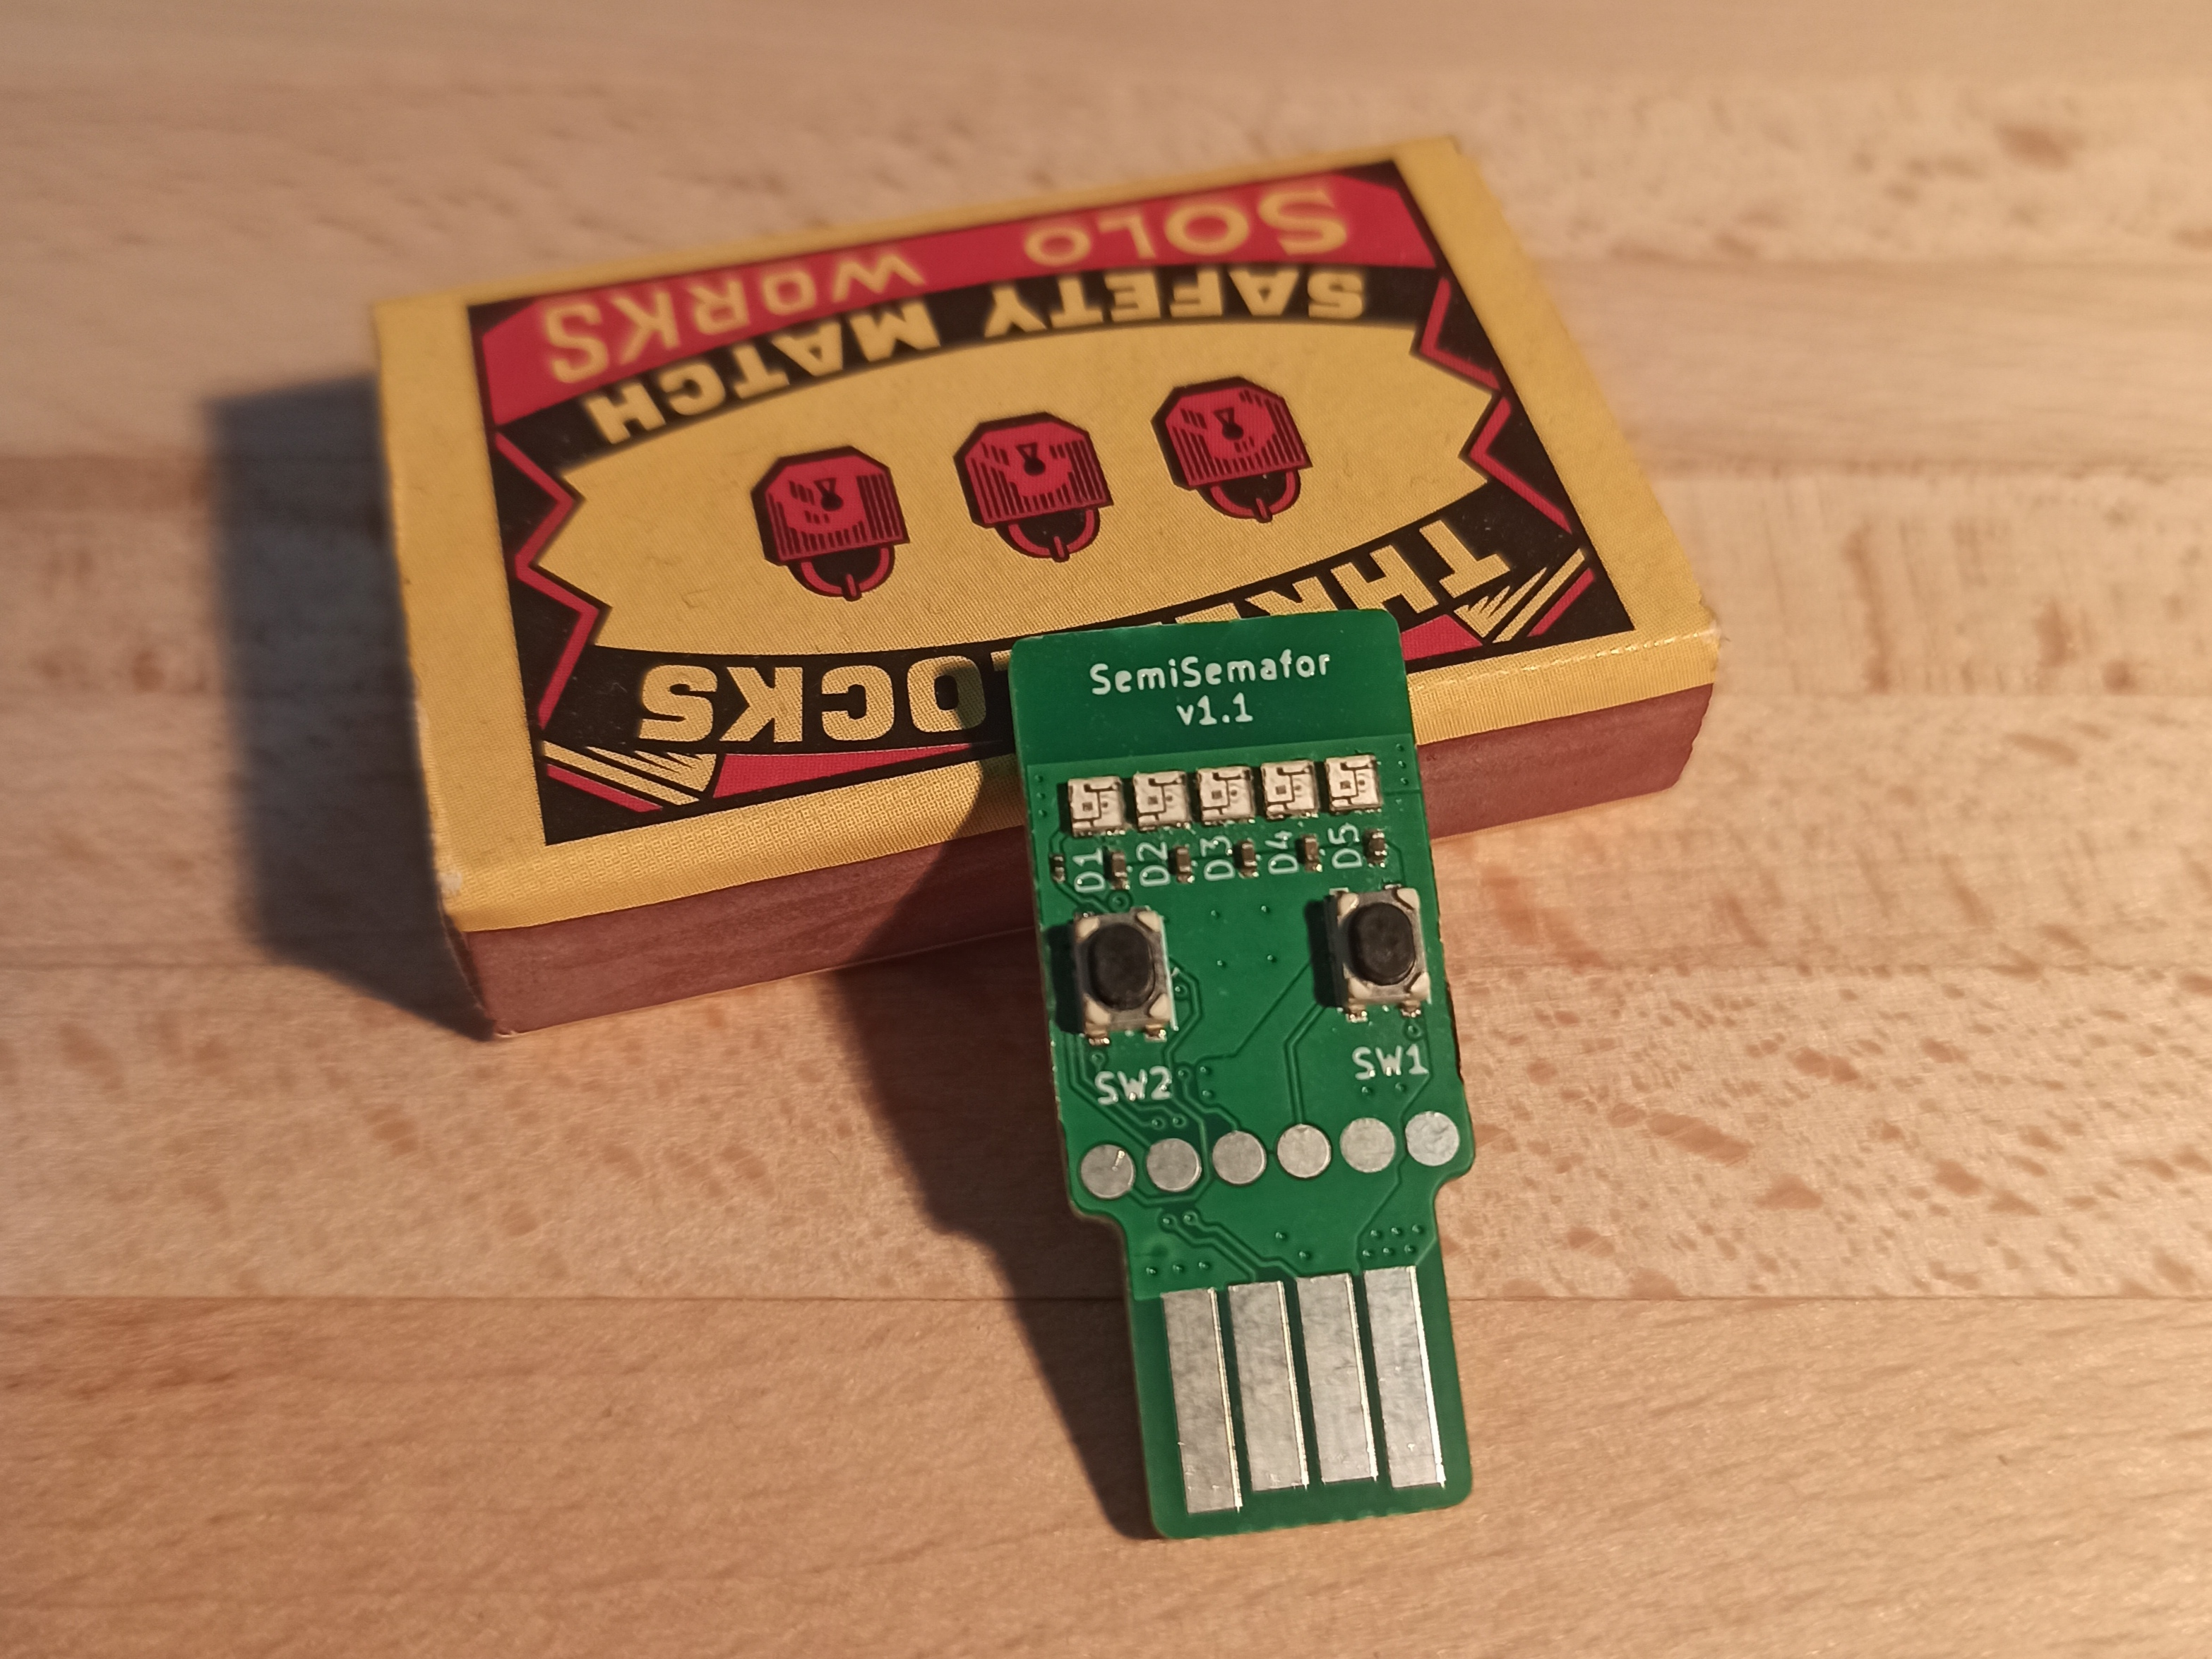
\includegraphics[width=0.8\textwidth]{text/TeoretickyUvod/AplikaceHernichZarizeni/img/1702085190411.jpg}
    \caption{Zařízení SemiSemafor}
    \label{fig:SemiSemafor}
\end{figure}

\subsection{Využití zařízení SemiSemafor}
SemiSemabor je využitelný například ve hře s názvem Duchové.


\section{Požadavky na zařízení}
Z~potřeb popsaných her nám vyplývají požadavky na zařízení.
Tato zařízení lze rozdělit na statická a~dynamická, podle toho, zda je má hráč nosit všude s~sebou nebo s~nimi jen interaguje na nehybném stanovištích.

\subsection{Dynamická zařízení}
Dynamická zařízení jsou ta, která má hráč nosit s~sebou.
Tato zařízení by tedy měla být co nejmenší a~nejlehčí, aby hráči nepřekáželo při pohybu.
Zároveň by měla být co nejlevnější, aby se dalo nasadit v~dostatečném množství.
Potřebuje také světelný výstup pro zobrazování herních stavů a~jednoduchý vstup pro ovládání. 

\subsection{Statická zařízení}
Statická zařízení jsou ta, u~nichž nepředpokládáme, že je bude hráč nosit s~sebou.
To ovšem neznamená, že mohou být libovolně velká a~těžká, pořád je potřeba, aby bylo snadné je přesunout z~místa na místo.
Stejně jako dynamická zařízení potřebují světelný výstup, aby bylo možno signalizovat herní stav a~reagovat na hráče.
Také je potřeba vstup, na což většinou stačí obyčejná tlačítka.
Problém je ale určit jaké a~kolik jich bude potřeba.
Některé hry vyžadují třeba jen jedno, ale takové, aby se do něj dalo co nejpohodlněji praštit v~běhu, protože je zrovna cílem ke stanovišti co nejrychleji doběhnout jako u~třeba u~hry King of the hill \ref{KOTH}.
Jiná hra může vyžadovat tlačítek víc, ale už není potřeba, aby byly tak velké, protože hráč při jejich používání nebude tak akční, ale bude třeba zadávat heslo, jako u~hry Špionská síť \ref{SpionskeSite}.
Univerzálnější je tedy nepoužívat tlačítka, ale nějaký systém, který se dá softwarově přizpůsobit.
Příkladem může být dotyková plocha, která se dá softwarově rozdělit na různé oblasti sloužící jako tlačítka a~i během hry se tak dá počet tlačítek měnit.
Další důležitou vlastností je možnost komunikace s~ostatními zařízeními, která do hry přináší novou možnost jak stanoviště propojit a~také pohodlnou metodu jak stanoviště nastavit přes telefon.
V~neposlední řadě je vhodné mít zvukový výstup, který může být použit např. jako potvrzení zadaného hesla, nebo odezva na prostý klik na dotykovou plochu.

Aby ale bylo možné zařízení použít v~různých hrách, je potřeba aby bylo možné ho přizpůsobit konkrétním potřebám.
Z~toho důvodu považujeme za vhodné k~základnímu zařízení moci připojit modul pro konkrétní herní mechaniky.

Z~toho nám tedy plyne diagram \ref{fig:diagram_zanoreni_0}.
\begin{figure}[h]
    \centering
    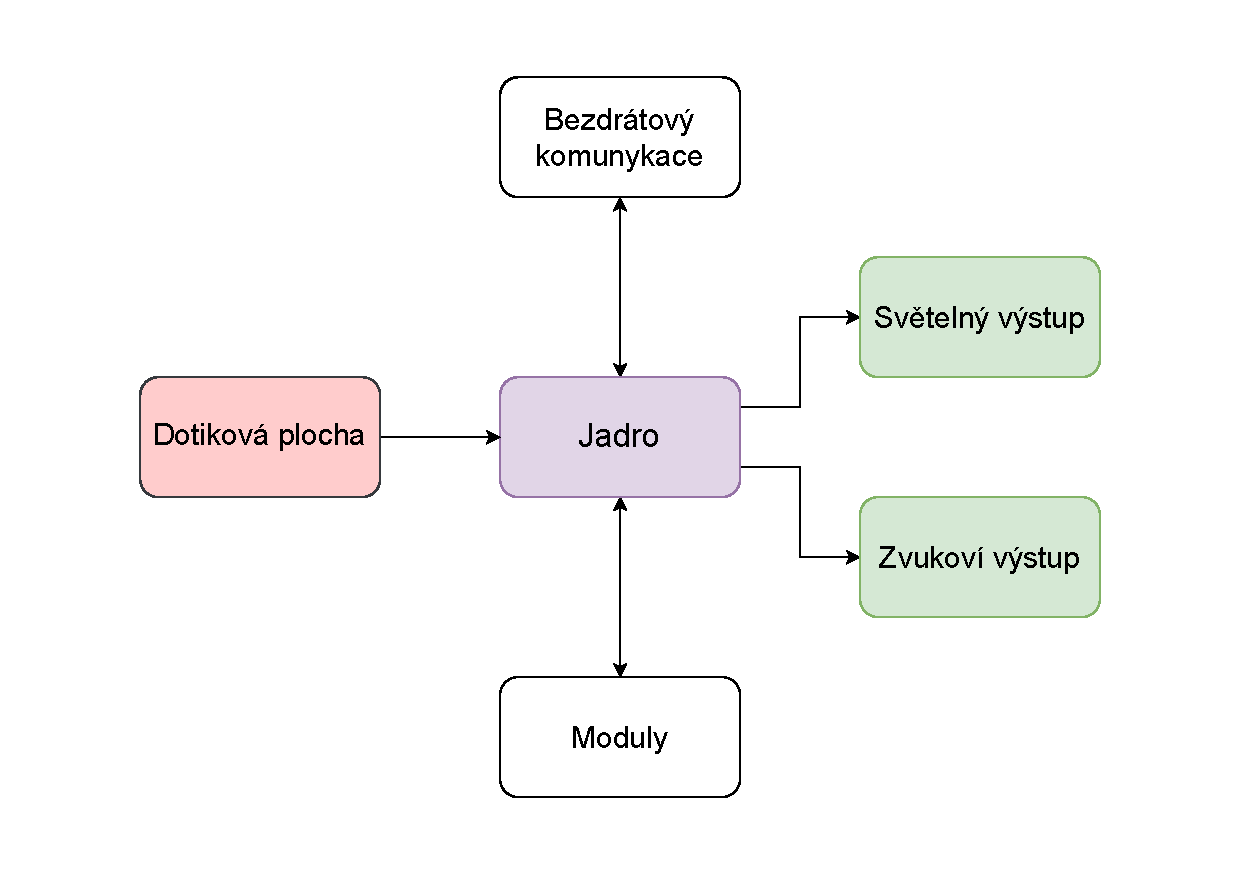
\includegraphics[width=0.65\textwidth]{text/TeoretickyUvod/AplikaceHernichZarizeni/diagram/zanoreni_0.pdf}
    \caption{Úvodní blokové schéma zařízení}
    \label{fig:diagram_zanoreni_0}
\end{figure}

Co se světelného výstupu týče, na signalizaci různých stavů je vhodné používat různé barvy světel.
% Jaký vzhled by ale měl mít zdroj barevného světla na podobném zařízení?
Jak je vysvětleno v~následující části \ref{VyuzitiTelefonu}, není potřebné suplovat grafický display, za tímto účelem se dá použít propojení s~telefonem.
Informace, kterou zařízení bude často poskytovat, je čas a~směr, např. čas do konce kola nebo směr k~dalšímu úkolu.
Podobné informace se dají elegantně zobrazit na kruhu.
%Protože má být stanoviště pohodlně čitelné z~blízky i~viditelné z~větší vzdálenosti, je tedy otázkou, zda použít jen jeden kruh, tak aby byl dostatečně viditelný, nebo jich použít více. %%TODO: otázka co s~totu otázkou?
Je vhodné zobrazování rozdělit na dva režimy, čtení na dálku a~čtení na blízko.
Pro čtení na blízko je cílem přímá interakce se zařízením, např. u~zadávání hesla.
Čtení na dálku je naopak určeno pro předávání informací hráči, když právě přímo neinteraguje se stanovištěm, např. který tým má zrovna povolený přístup do zařízení.
Proto je vhodné mít kruhů více, aby bylo možné zobrazovat tyto informace na různých kruzích, které mohou navíc být svému účelu přizpůsobeny.
Jeden kruh tak může svítit jen jedním směrem, aby ho hráč viděl celý najednou pro blízkou interakci, zatímco druhý kruh může svítit do všech stran, aby byl vidět z~co nejvíce míst.

Potřeba propojení s~telefonem nám omezuje možnosti co se týče bezdrátové komunikace, protože telefony jsou většinou vybaveny Bluetooth a~WiFi.
Také se v~telefonech rozšiřuje NFC, to je však pro tuto aplikaci z~důvodu krátkého dosahu nevhodné.

Posledním systémem, který je třeba zmínit, je zvukový výstup.
Protože většinou stačí jen jednoduchá zvuková odezva, není potřeba plnohodnotný zvukový systém.
Pro hry, které budou potřebovat přehrávat libovolnou nahrávku, bude samostatný zvukový modul, případně je možnost nahrávku přehrát přes uživatelův telefon.
V~základním zařízení je proto potřeba jen jednoduchý bzučák, například jako odezva na kliknutí.

Můžeme tedy diagram upravit na \ref{fig:diagram_zanoreni_1}.
\begin{figure}[h]
    \centering
    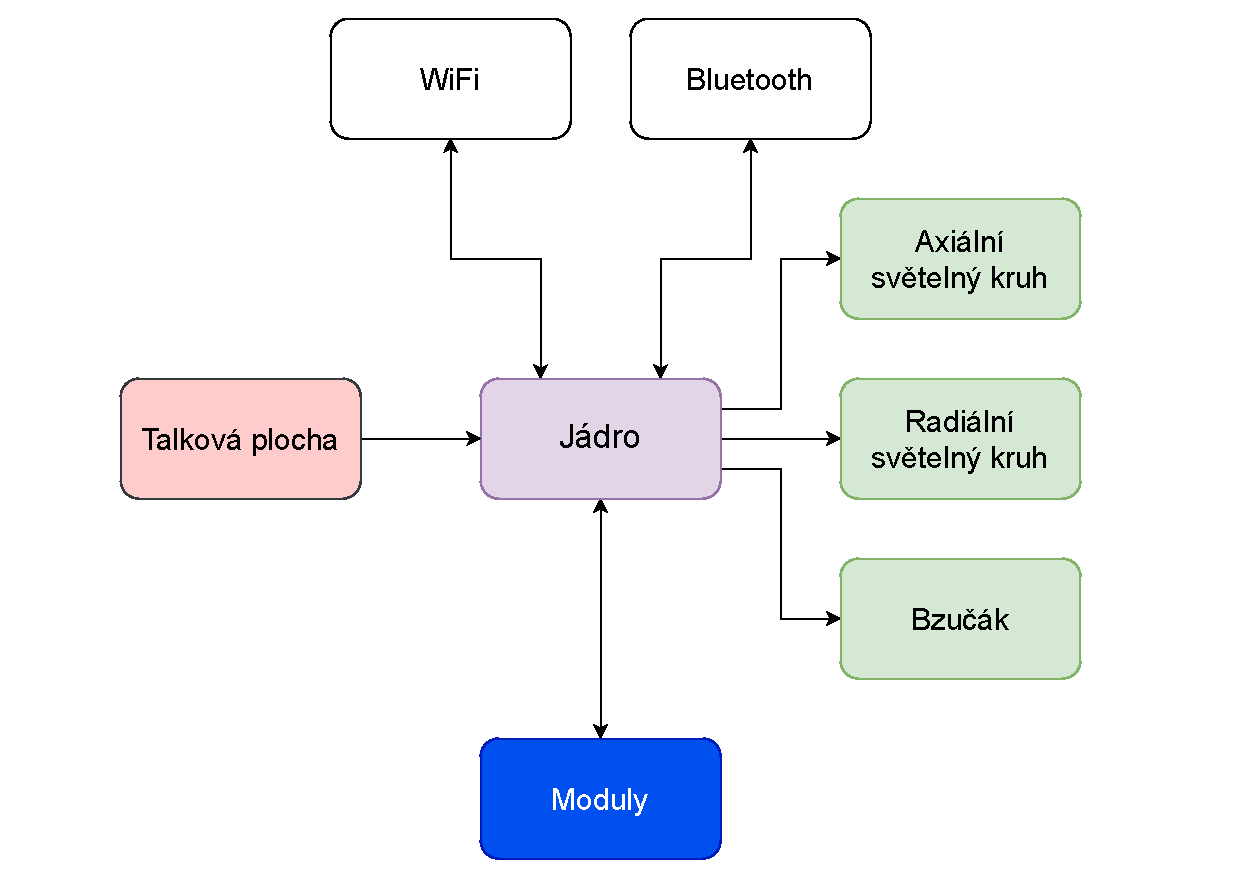
\includegraphics[width=0.65\textwidth]{text/TeoretickyUvod/AplikaceHernichZarizeni/diagram/zanoreni_1.pdf}
    \caption{Základní blokové schéma zařízení}
    \label{fig:diagram_zanoreni_1}
\end{figure}

Celé zařízení by také mělo být alespoň částečně voděodolné, aby se dalo použít třeba i~za deště.

\subsection{Využití telefonu \label{VyuzitiTelefonu}}
Podstatný fakt je, že prakticky všichni u~sebe dnes mají chytrý telefon, čehož můžeme využít.
Nemá proto velký význam, aby naše statické nebo dynamické zařízení suplovalo funkce telefonu.
Např. grafický výstup typu display proto v~podobném zařízení není potřeba, a~v tomto směru už odvádí telefon naprosto dostatečnou práci.
Pokud by tedy v~rámci hry bylo potřeba například předat hráči text nebo obrázek, může jej zařízení poslat uživateli na telefon.
Telefon by se tedy dal zařadit mezi dynamická zařízení.
Možnost propojení s~telefonem je také velmi významná při nastavování hry.
Díky telefonu totiž zařízení nepotřebuje uživatelské rozhraní přizpůsobené k~nastavování, ale prostě se vše nastaví z~telefonu.

Někdy by se mohlo zdát, že herní stanoviště vlastně ani není potřeba a~stačila by mobilní aplikace.
Ale přestože je mobil ve hrách dobře využitelný, jsou aplikace, na které jednoduše vhodný není.
Pokud má hráč například ze stanoviště získat fyzický objekt, mobil neposlouží.
Pro hráče ani organizátory také nemusí být zrovna komfortní před hrou zařizovat, aby měli všichni nainstalovaný správný software.
% Telefon také není například na stanovišti v~lese dobře viditelný.
V~neposlední řadě jde také o~jistý "cool efekt", který běžné zařízení jako mobil nebo třeba tablet neposkytne. %%TODO: tohle chce nějak přeformulovat


% Zařízení určené primárně pro outdoorové hry bychom mohli rozdělit na dvě skupiny, statické a~dynamické, protože jsou na tyto skupiny kladeny výrazně jiné požadavky.
% Dynamická zařízení jsou ta, která může uživatel pohodlně nosit s~sebou.
% Do dynamických zařízení by se tak dal zařadit právě i~telefon, ten však může být z~různých důvodu nevhodný a~proto i~tato zařízení dává smysl navrhnout specificky pro hry.
% Statické zařízení je naopak zařízení, u~kterého se nepředpokládá, že jej bude hráč nosit s~sebou.
% Přesto by mělo být jednoduše přenositelné, má jít o~stanoviště, které se pohodlně donese na své místo a~během hry se s~ním nebude pohybovat.
% Takové zařízení by tedy mělo být dobře viditelné a~splňovat požadavky, které na něj konkrétní hra klade. %%TODO: tohle chce nějak přeformulovat?
% Požadavky různých her můžou být ale dost rozdílné, častým požadavkem je něco uchovávat a~např. po zadání hesla hráči vydat.
% Hra ale taky může vyžadovat, aby bylo zařízení schopné přehrát audio nahrávku nebo naopak pořídit záznam. %%TODO: tohle chce nějak přeformulovat?
% Z~těchto důvodů považujeme za vhodnější zařízení koncipovat jako základní řídící jednotku, která je samostatně funkční a~použitelná při hře, ale ke které se dají jednoduše připojit moduly pro konkrétní herní mechaniky.

% \section{Základní řídící jednotka}
% % Z toho plyne otázka, jaká funkcionalita je potřebná v základním zařízení?
% Asi žádný systém, se kterým hráč přímo interaguje, není nutný v každé hře.
% Jde tedy o to vybrat takové systémy, které svými nároky nepřevýší užitečnost při hrách.
% Ze zkušeností považujeme za nejzákladnější systém nějaký světelný výstup, ten dokáže většinu her velmi příjemně ozvláštnit.
% Většinou je nezbytný i uživatelský vstup, na což většinou stačí obyčejná tlačítka.
% Problém je ale určit jaké a kolik jich bude potřeba.
% Některé hry vyžadují třeba jen jedno, ale takové, aby se do něj dalo co nejpohodlněji praštit v běhu, protože je zrovna cílem ke stanovišti co nejrychleji doběhnout.
% Jiná hra může vyžadovat tlačítek víc, ale už není potřeba, aby byly tak velké, protože hráč při jejich používání nebude tak akční, ale bude třeba zadávat výsledek logického úkolu.
% Univerzálnější je tedy nepoužívat tlačítka, ale nějaký systém, který se dá softwarově přizpůsobit.
% Příkladem může být dotyková plocha, která se dá softwarově rozdělit na různé oblasti sloužící jako tlačítka a i během hry se tak dá počet tlačítek měnit.
% Další důležitou vlastností je možnost komunikace s ostatními zařízeními, která do hry přináší novou možnost jak stanoviště propojit a také pohodlnou metodu jak stanoviště nastavit přes telefon.
% V neposlední řadě je potřeba zvukový výstup, který může být použit např. jako potvrzení zadaného hesla.

% Z toho nám tedy plyne diagram \ref{fig:diagram_zanoreni_0}.
% \begin{figure}[h]
%     \centering
%     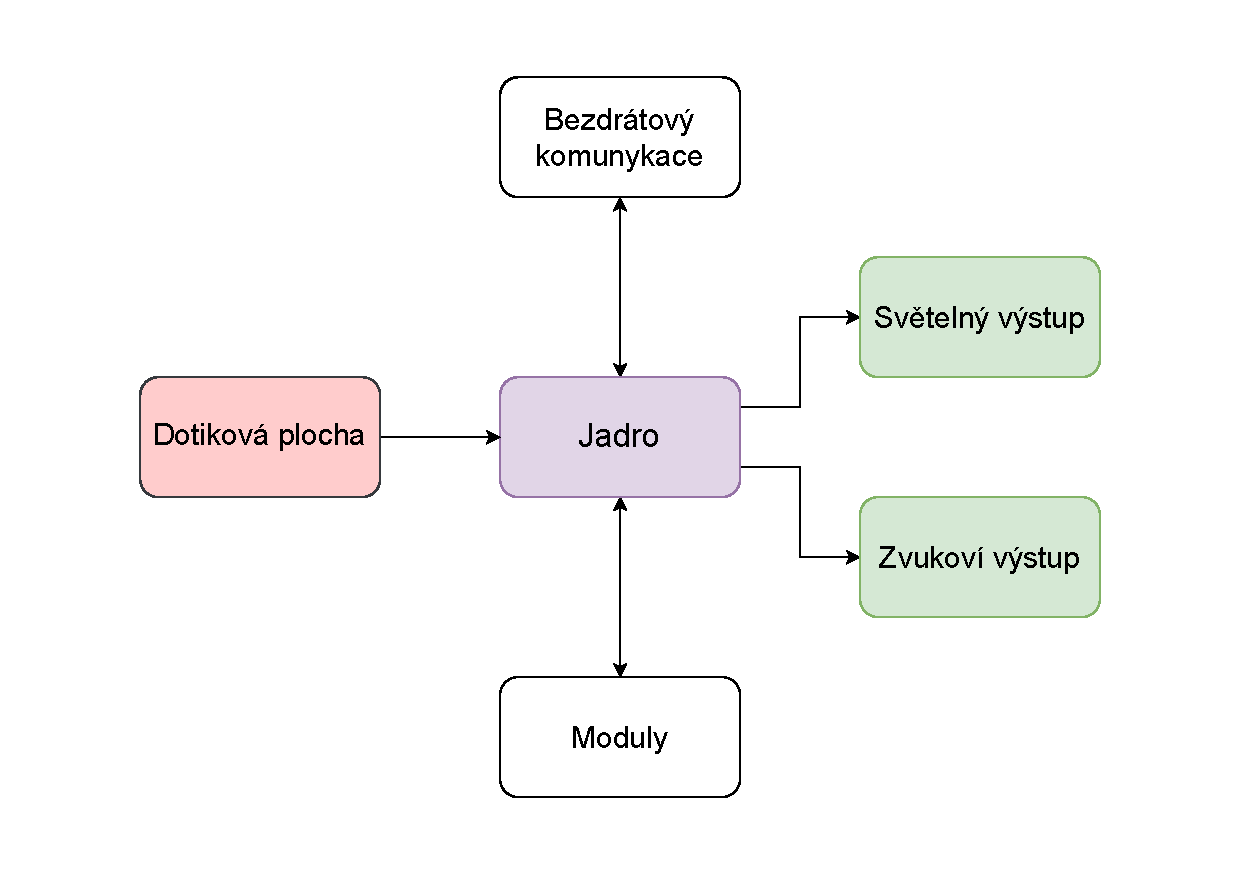
\includegraphics[width=0.65\textwidth]{text/TeoretickyUvod/AplikaceHernichZarizeni/diagram/zanoreni_0.pdf}
%     \caption{Úvodní blokové schéma zařízení}
%     \label{fig:diagram_zanoreni_0}
% \end{figure}

% \newpage

Co se světelného výstupu týče, na signalizaci různých stavů je vhodné používat různé barvy světel.
% Jaký vzhled by ale měl mít zdroj barevného světla na podobném zařízení?
Jak je uvedeno výše, není potřebné suplovat grafický display, za tímto účelem se dá použít propojení s telefonem.
Informace, kterou by zařízení mohlo často poskytovat je čas a směr, např. čas do konce kola nebo směr k dalšímu úkolu.
Podobné informace se dají elegantně zobrazit na kruhu.
Protože má být stanoviště viditelné i z větší vzdálenosti, je tedy otázkou, zda použít jen jeden kruh, tak aby byl dostatečně viditelný, nebo jich použít více. %%TODO: otázka co s totu otázkou?
Zobrazování pracuje ve dvou režimech, čtení na dálku a čtení na blízko.
Pro čtení na blízko je cílem přímá interakce se zařízením např. už zmiňované zadávání hesla.
Čtení na dálku je naopak určeno pro předávání informací hráči, když právě přímo neinteraguje se stanovištěm, např. který tým má zrovna povolený přístup.
Proto je vhodné mít kruhů více, aby bylo možné zobrazovat tyto informace na různých kruzích, které mohou navíc být svému účelu přizpůsobeny.
Jeden kruh tak může svítit jen jedním směrem, aby ho hráč viděl celý najednou pro blízkou interakci, zatímco druhý kruh může svítit do všech stran, aby byl vidět z co nejvíce míst.

Potřeba propojení s telefonem nám omezuje možnosti co se týče bezdrátové komunikace, protože telefony jsou většinou vybaveny Bluetooth a WiFi.
Také se v telefonech rozšiřuje NFC, to je však pro tuto aplikaci z důvodu krátkého dosahu nevhodné.

Posledním systémem, který je potřeba, je zvukový výstup.
Protože většinou stačí jen jednoduchá zvuková odezva, není potřeba plnohodnotný zvukový systém.
Pro hry, které budou potřebovat přehrávat nějakou nahrávku, bude samostatný zvukový modul, případně je možnost nahrávku přehrát přes uživatelův telefon.
V základním zařízení je proto potřeba jen jednoduchý bzučák, například jako odezva na kliknutí.

Můžeme tedy diagram upravit na \ref{fig:diagram_zanoreni_1}.
\begin{figure}[h]
    \centering
    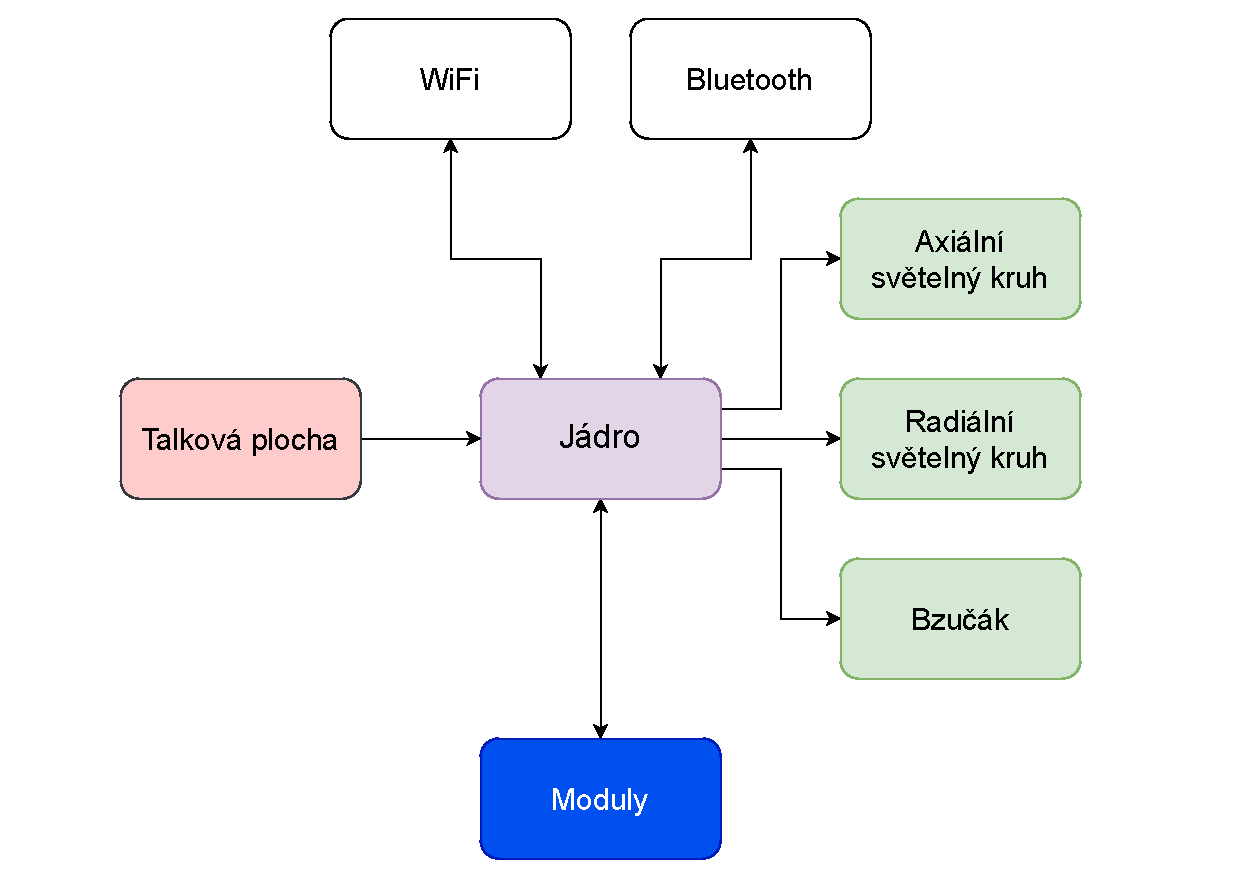
\includegraphics[width=0.65\textwidth]{text/TeoretickyUvod/AplikaceHernichZarizeni/diagram/zanoreni_1.pdf}
    \caption{Základní blokové schéma zařízení}
    \label{fig:diagram_zanoreni_1}
\end{figure}

Celé zařízení by také mělo být alespoň částečně voděodolné, aby se dalo použít třeba i za deště.

\vspace{-10mm}
\section{Moduly}
Základní řídící jednotka je tedy schopná poskytnout základní funkce, které jsou potřeba pro většinu her.
Některé hry ale mohou vyžadovat nějakou specifickou funkci, kterou základní zařízení nedokáže poskytnout.
Proto je vhodné, aby bylo možné k~základnímu zařízení připojit externí moduly, bez kterých by se konkrétní hry neobešly.

\subsection{Modul dvířka}
Asi nejzákladnější modul jsou dvířka.
Dvířka přidávají uzamykatelné přihrádky.
Do stanoviště se tak dá uzamknout předmět potřebný ke splnění úkolu, který hráči získají například po zadání hesla nebo vyřešení zadaného úkolu.
Přihrádky pak mohou sloužit pro více týmů nebo třeba uchovávat více objektů do různých částí hry.

Pro jednoduchost jsou dvířka zamykána magneticky.
Vrátka jsou uchycena na kloubu ve své horní části a~v dolní části se nachází magnet.
Pod dnem přihrádky se pak nachází servomotor vybavený druhým magnetem, který tak může dvířka přitáhnout nebo odpudit.
Toto řešení neposkytuje bezpečné uzamčení přihrádky, vrátka se dají vypáčit někdy i~nehtem, ale pro účely her je to dostačující řešení.
Aby bylo možné ověřit, zda se vrátka dovřela, je vedle serva i~spínač, který se sepne při dovření vrátek.
Z~tohoto řešení vyplynula další možnost jak modul dvířek využít.
Vrátka se při odemčení pootevřou, a~protože jsou v~tu chvíli jen odpuzována magnetem, je možné je stlačit zpět a~sepnout tak spínač.
Tento fakt se ukázal být užitečný, protože tak vznikla velká pohodlná tlačítka.
Struktura tohoto modulu je vidět na diagramu \ref{fig:diagram_dvirka} ve verzi se čtyřmi přihrádkami.

\begin{figure}[h]
    \centering
    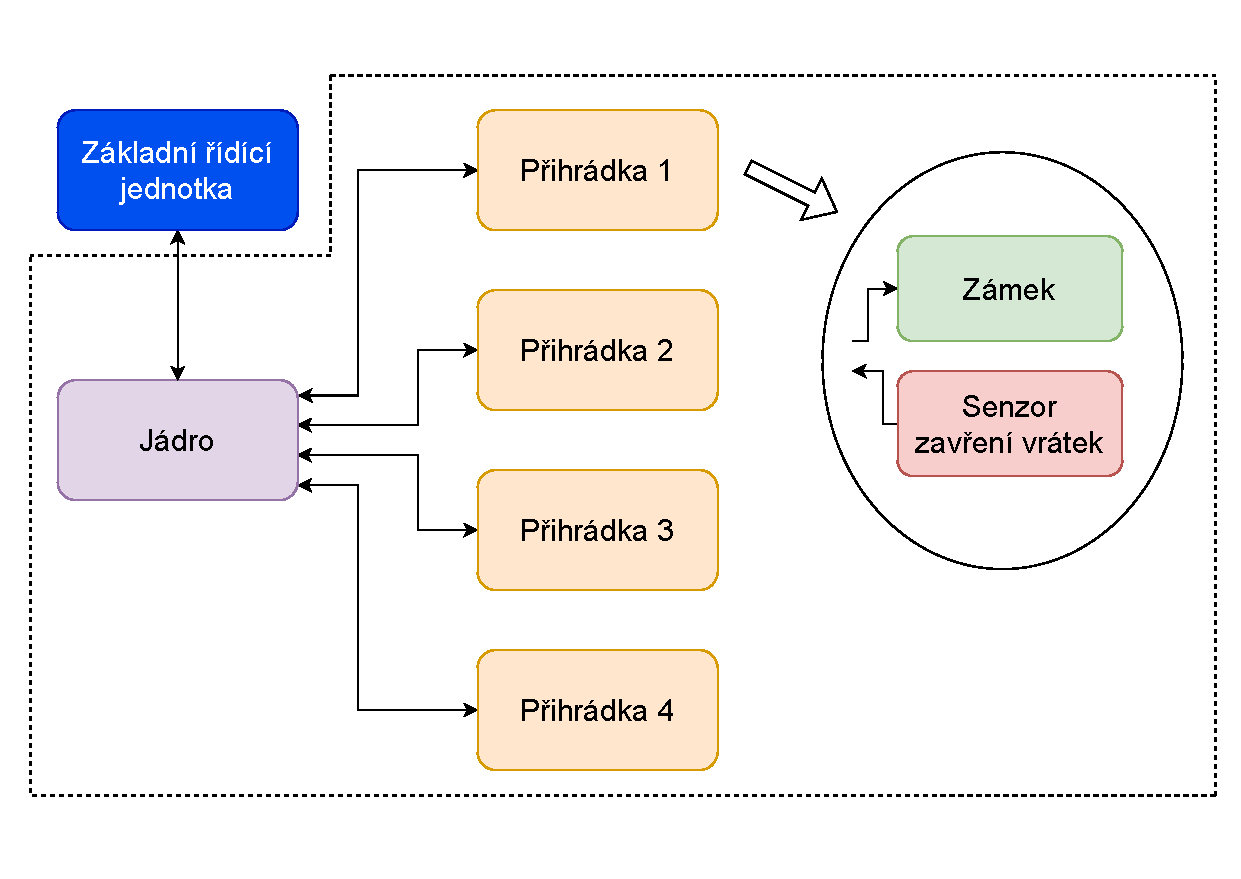
\includegraphics[width=0.65\textwidth]{text/TeoretickyUvod/AplikaceHernichZarizeni/diagram/Dvirka.drawio.pdf}
    \caption{Blokové schéma modulu dvířka}
    \label{fig:diagram_dvirka}
\end{figure}
 
Jednoduchá hra, která vyžaduje modul dvířka, je např. hra Maják. %%TODO: vymyslet lepčí název tohle se  mi moc nepozdává (je to název z~her od Petra na první lucerný v~roce 2021)
V~této hře jsou hráči rozděleni do týmů a~každý tým má svou barvu, od které je odvozena konkrétní přihrádka. 
Týmy mají za úkol získat co nejvíc sad kartiček.
Na hřišti je několik automatických stanovišť s~modulem dvířka a~v každém z~nich je nějaký typ kartičky.
Každé stanoviště během hry umožňuje přístup vždy právě jednomu z~týmů, který v~pravidelném intervalu mění, a~čas do změny reprezentuje na jednom z~kruhů.
Při startu hry si každé stanoviště náhodně vybere tým, kterým začne, a~následně se už drží konstantního pořadí.
Když někdo dorazí ke stanovišti ve chvíli, kdy je stanoviště zpřístupněné jeho týmu, a~klepne na tlakovou plochu, stanoviště mu vydá kartičku.
Stanoviště se týmu zpřístupní jen v~čase daného týmu a~navíc jen jednou za kolo.
Hráčům cíleně není představen celý mechanizmus výdeje kartiček, je jim řečeno jen, že se přihrádka otevírá klepnutím do tlakové plochy a~že je zajímají jen kartičky jejich barvy. 
Tým tedy musí spolupracovat nejprve na odhalení mechanizmu a~následně myslet jak zvítězit.

Podobná hra se buď dá hrát samostatně nebo může jít například jen o~metodu, jak získávat suroviny v~nějaké komplexnější hře.

\subsection{Zvukový modul}
Další plánovaný modul, který se dá připojit, je zvukový modul.
Hra, která vyžaduje zvukový modul, je například hra s~názvem Ticho.
Tato hra vyžaduje zároveň i~modul dvířka.
V~této hře stanoviště sleduje intenzitu zvuku v~okolí a~v momentě, kdy hluk klesne pod stanovenou úroveň, stanoviště otevře dvířka. 
% Ucastnikum není ovládání představeno a~musí tak na něj přijít samy.
Stanoviště je hráčům představeno jako "magická krabička"\- za čárou, ke které se nesmí proplížit, ale můžou ji ovlivnit z~dálky.
Úkolem hráčů tak je přijít na to, jak krabička funguje a~jak ji přesvědčí, aby se otevřela.

V~rámci zvukového modulu je i~možnost nahrávku přehrát.
Tato část zvukového modulu umožňuje intenzivnější vtažení hráče do hry s~příběhem.
Může jít například o~únikovou hru, při které se hráč ocitne v~oblasti neznámého bludiště a~jeho úkolem je najít cestu ven.
Při hledání může narazit na různá stanoviště, která mu nejprve přehrají nějakou část příběhu a~následně mu dají úkol nebo radu jak postupovat dál.

\subsection{Komunikační modul \label{sec:KomunikacniModul}}
Podstatným modulem je také komunikační modul, který umožňuje připojení k~mobilní síti a~tím i~komunikaci s~ostatními zařízeními na velkou vzdálenost.
Tento modul je potřeba například pro hru Boj o kopce.

V~této hře se na hřišti o~velké rozloze nachází několik automatických stanovišť.
Hráči jsou rozděleni do týmů a~každý tým má svou barvu a~své tlačítko na stanovišti označené barvou týmu.
V~hře je hlavním cílem získávat body pro svůj tým ovládnutím a~udržením stanovišť na rozsáhlém hřišti. 
Axiální světelný kruh zobrazuje rozdělení tlakové plochy na jednotlivá tlačítka týmů podle jejich barvy.
Zabrání stanoviště pak mohou hráči provést stiskem příslušného tlačítka. 
Získávání bodů se odehrává dvěma způsoby, ovládnutím stanoviště a~následným držením stanoviště pod kontrolou. 
Týmy mohou přebírat stanoviště od soupeřů, což přidává hře strategický rozměr. 
Výhodou je kontrolovat více stanovišť najednou, což umožňuje rychlejší získávání bodů a~zvyšuje šanci na vítězství.
Komunikační modul je tu potřebný pro vyhodnocování hry.
Stanoviště totiž musí být schopné komunikovat s~centrálním serverem, který vyhodnocuje hru a~zobrazuje její průběh.
Tato hra je původně navržena pro airsoftové hráče na hřiště v~Mokrá-Horákov o~rozloze \(6.7\-[ha]\) \cite{MokraHorakov}.
V~takovém prostředí tedy komunikace pomocí WiFi či Bluetooth nedostačuje, protože stanoviště mohou být i~několik set metrů od sebe.

\subsection{Výběr bezdrátové komunikace dlouhého dosahu \label{sec:TypVzdaleneKomunikace}}
Pro komunikaci na vzdálenosti v~řádu jednotek kilometrů se nabízí asi jen dvě základní možnosti, LoRa a~mobilní síť.
Ještě počátkem roku 2023 by byla i~třetí možnost, Sigfox, ale jeho síť byla v~ČR vypnuta \cite{SigfoxKonci}.

LoRa je technologie určená pro komunikaci na dlouhé vzdálenosti s~malou spotřebou a~datovou propustností.
Pracuje v~bezlicenčním pásmu a~není tedy třeba platit za provoz.
Její dosah je i~v zastavěné oblasti v~řádu kilometrů \cite{LoRaSEMTECH}, a~za ideálních podmínek na přímou viditelnost i~přes sto kilometrů \cite{LoRaEMAN}. 
Nevýhoda LoRy je ale malá datová propustnost ještě snížená omezením času provozu na \(1\-\%\)\cite{LoRaEMAN}.

Mobilní síť má v~porovnání s~LoRou výrazně větší datovou propustnost, ale na druhou stranu je třeba platit za provoz a~je méně energeticky úsporná.
Například \\NB-IoT je energeticky asi o~třetinu náročnější než LoRa.
Přesto je dostatečně úsporná, aby bylo zařízení, které tuto technologii využívá, schopno běžet na baterii přes deset let \cite{LoRaVSNB-IoT}.
Energetická náročnost tedy není problém a~vyšší datová propustnost společně s~připojením na internet je významnější výhoda než bezplatný provoz u~LoRy.
Další výhodou LoRy by mohla být nezávislost na pokrytí mobilních sítí, ale vzhledem k~tomu, že pokrytí NB-IoT sítě je v~ČR údajně \(100\-\%\)\cite{NB-IoTPokryti}, není tento fakt důležitý. 

% \section{Dynamických zařízení}
% U některých her je potřeba, aby měl hráč zařízení, které bude moci nosit s sebou a které mu při hře bude sloužit jako identifikace nebo nástroj pro plnění úkolů.
Takové zařízení by mělo být co nejmenší a co nejlehčí, aby hráče při hře nezdržovalo.
Navíc by mělo být co nejlevnější, aby tolik nevadilo, když jej některý hráč třeba ztratí, což se přeci jen může stát.
Mimo to toto zařízení musí být schopno zobrazit svůj stav a převzít od uživatele jednoduchý pokyn.

% Rozhodli jsme, že toto zařízení bude svůj stav zobrazovat pomocí pěti inteligentních RGB LED a jako vstup mu budou sloužit dvě tlačítka.
% Abychom nemuseli řešit napájení, má toto zařízení USB konektor a je určeno k napájení powerbankou.
% Toto zařízení jsme nazvali SemiSemafor a jeho vzhled je na obrázku \ref{fig:SemiSemafor}.

% \begin{figure}[h]
%     \centering
%     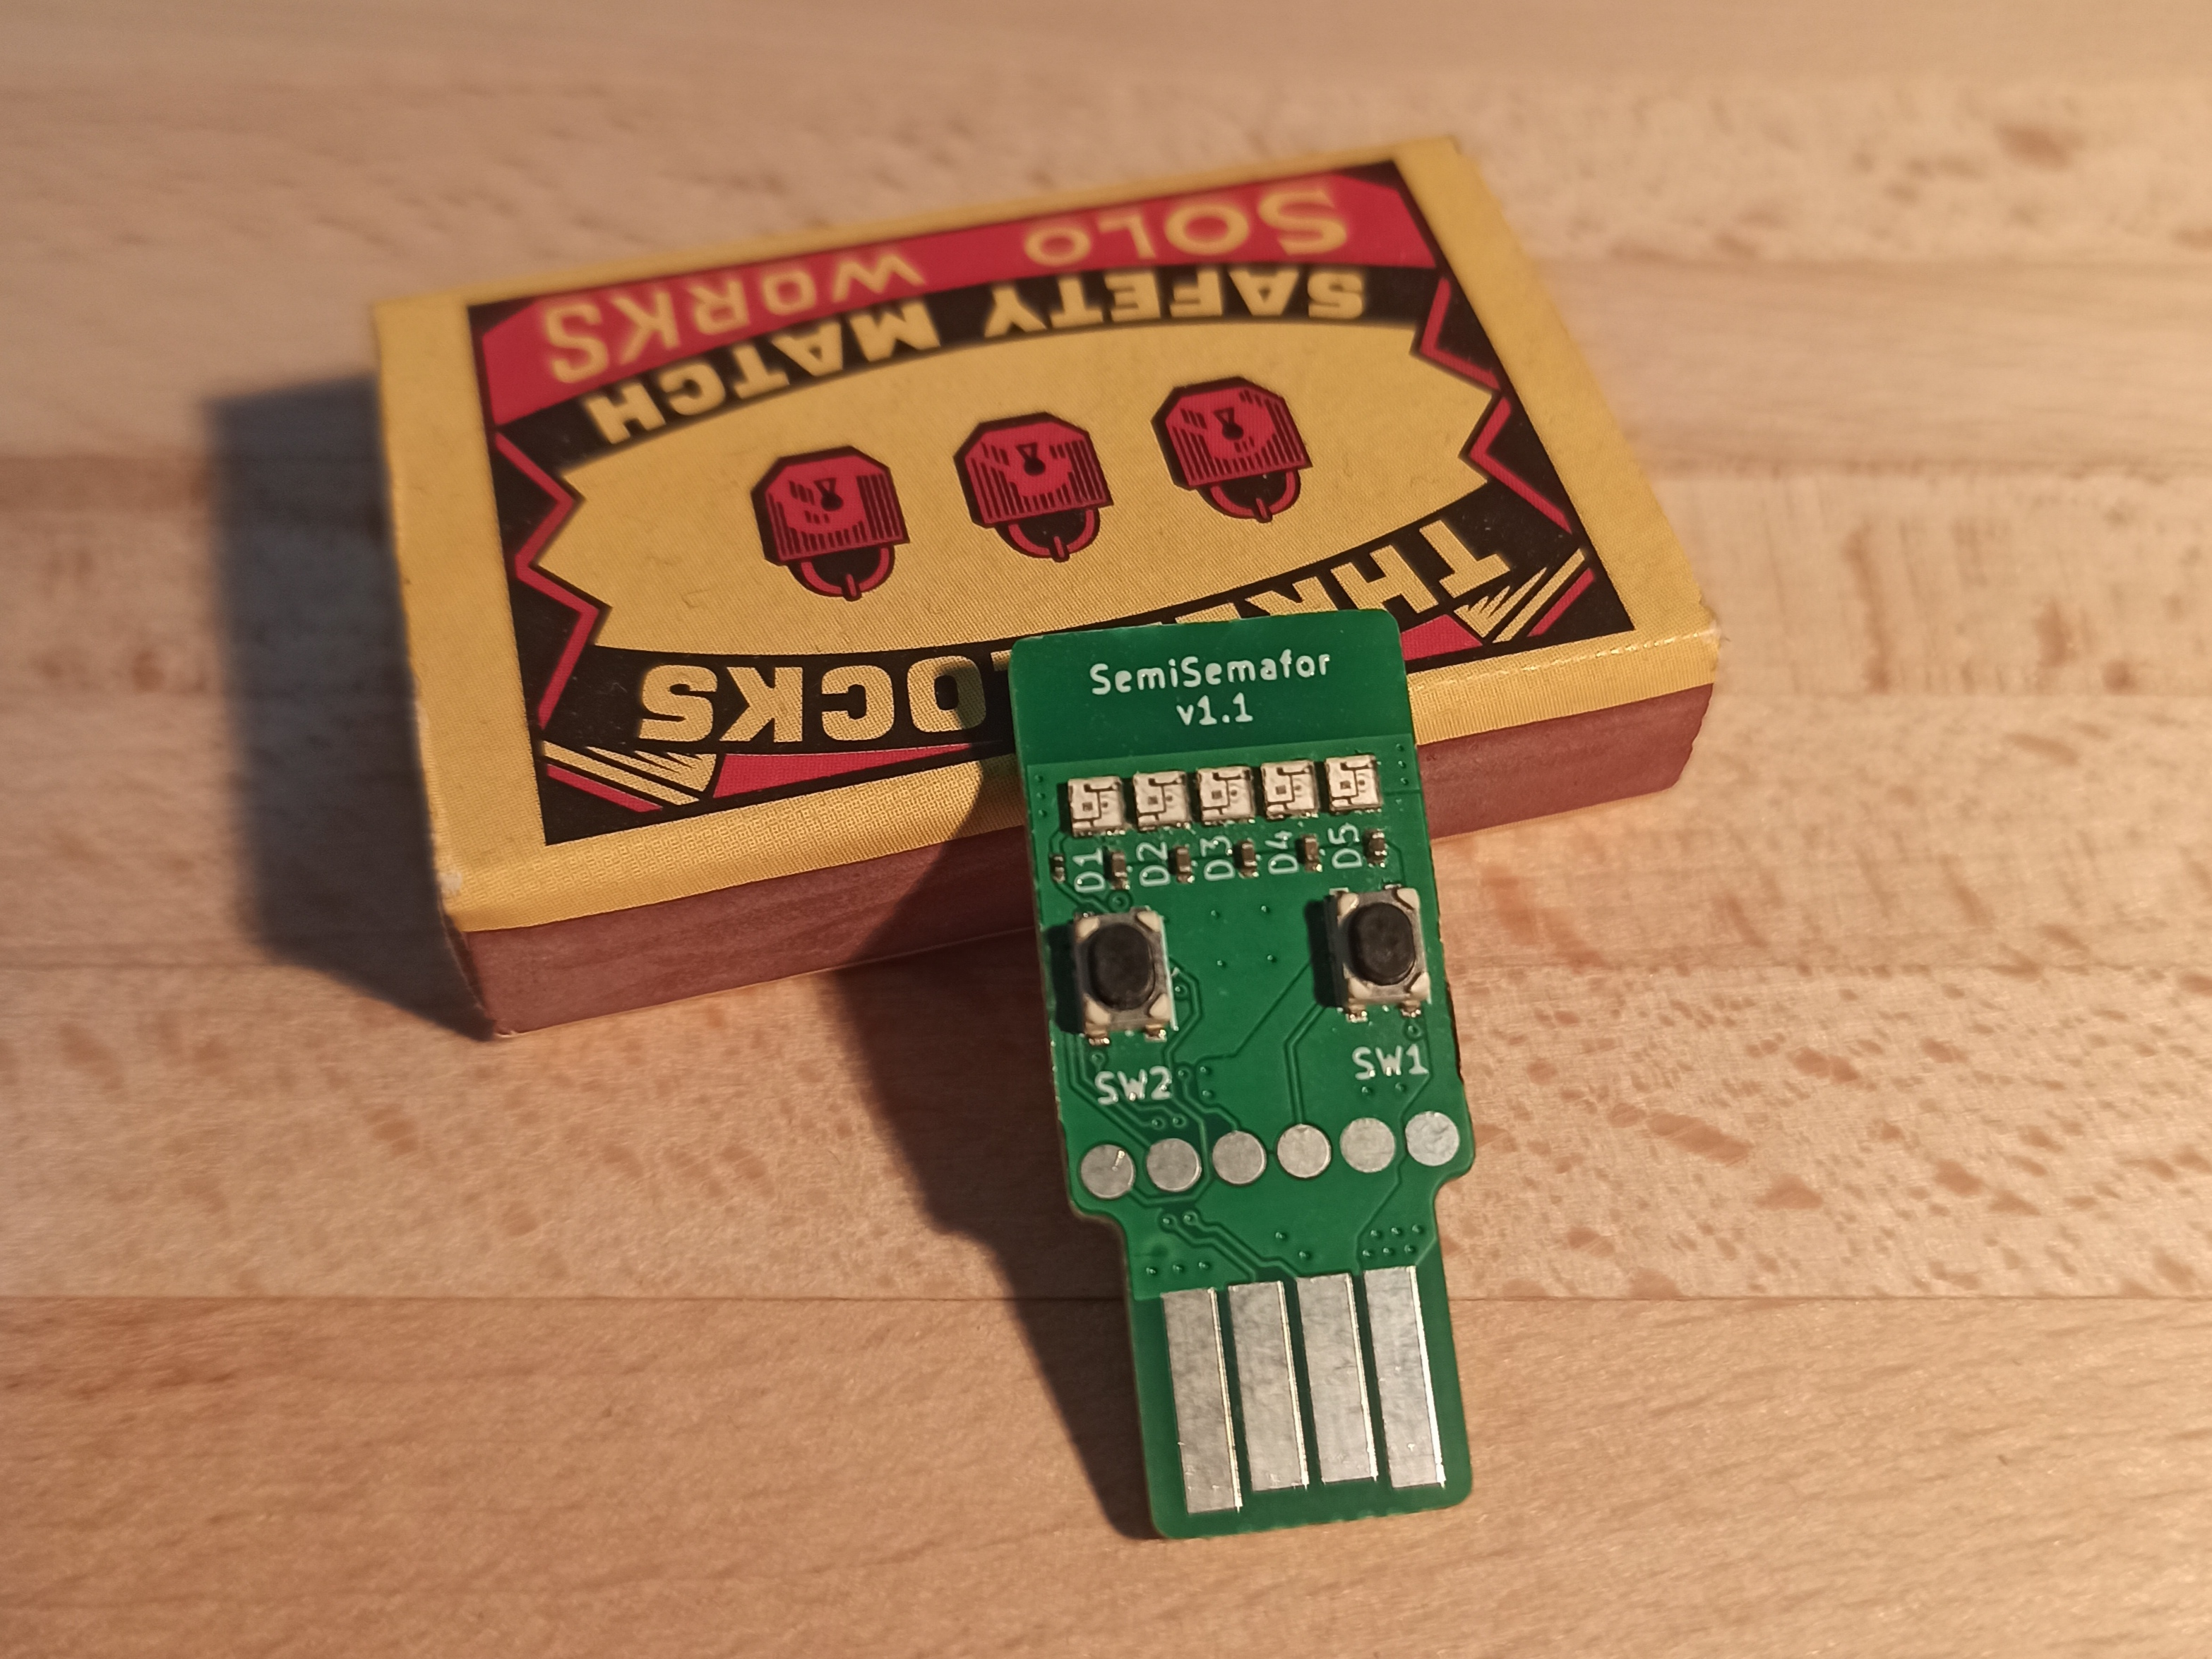
\includegraphics[width=0.8\textwidth]{text/TeoretickyUvod/AplikaceHernichZarizeni/img/1702085190411.jpg}
%     \caption{Zařízení SemiSemafor}
%     \label{fig:SemiSemafor}
% \end{figure}

% \subsection{Využití zařízení SemiSemafor}
% SemiSemafor je využitelný například ve hře s názvem Duchové.
% Nabiječa, artefakt, SemiSemafor = učastnická lucernička
% učastník dojde k nabiječce, nabije ce a u artefaktu předali energii
% lucerničky se samovibijí,
% když zmáčkneč tlačítko mužeš nabijet artefakt ale když uněj nejseš a lucernička se vybije dvakrát rychleji a odpuzuje duchy (svítí u toho bíle)
% duchová mají taky zařízení (Semiho) když drží tlačítko vybijí lucerničku i artefakty v okolí (nesvítí u toho)
% víc lidí muže naráz nabijet
% když duch chytí hráče, hráč si musí na pět minut ze hry, u nabíječky je respoun
% cílem je nabít všech tt artefaktů

% potenciálně by duchové mohli ke své činnosti potřebovat energiiž

%%% Vložení souboru 'text/vysledky' s popisem vysledků práce
% (rozdělte na více souborů či kapitol, pokud je vhodné)
\chapter{Návrh dynamického zařízení}
Uživatelským požadavkem je dynamické zařízení sloužící například jako identifikátor hráče, nebo jako herní nástroj.
Mělo by ale být sto zastat i~roli statického zařízení, pro případy her na delších výletech, kde by bylo nepraktické nosit s~sebou velké zařízení.
Vyžaduje tedy dostatečnou mobilitu, aby uživateli nepřekáželo v~pohybu.
Zároveň by zařízení mělo být co nejlevnější, pro případ ztráty nebo poškození.
Z~toho plynou požadavky na velikost výslednou konstrukci zařízení.

Zařízení by mělo být schopno komunikovat s~ostatními zařízeními, ať už statickými nebo dynamickými.
Potřebuje také světelný výstup pro zobrazování herních stavů a~jednoduchý vstup pro ovládání.

Vstup bude realizován pomocí dvou tlačítek.

Světelný výstup bude realizován pomocí pěti inteligentních RGB LED.
Číslo pět bylo zvoleno jako maximální množství, které se pohodlně vleze vedle sebe na desku plošných spojů o~šířce mikrokontroleru ESP32-C3-MINI-1 \cite{ESP32C3}.
ESP32-C3-MINI-1 byl vybrán jakožto nejlevnější mikrokontroler z~rodiny ESP32, který má zároveň Wi-Fi a~Bluetooth.

Abychom se vyhnuli elektronice řešící baterii, je napájení zajištěno pomocí USB-A konektoru a~powerbanky.

ESP32-C3-MINI-1 má stejně jako ESP32-S3 USB periferii, která se dá využít na programování zařízení.
I~tady je ale problém, že se tato metoda dá softwarově rozbít a~zařízení je proto vybaveno stejným programovacím konektorem jako ESP32-S3 na AHS.

% \section{Neočekávané problémy}
% První verce trpěla nečekaným problémem s~kmitajícími hranami řídícího signálu LEDek.
% Tento problém pravděpodobně nastal v~důsledku kombinace parazitních vlastnosti výstupního pinu mikrokontroleru, vstupního pinu LEDek a~příliš krátké dráhy.

% Signál tak začal oscilovat na frekvenci zhruba \(50\-[MHz]\) a~LEDky tak nebyly schopny signál rozpoznat.
% \begin{tikzpicture}
%     \begin{axis}[
%         xlabel={X},
%         ylabel={Y},
%     ]
%     \addplot table [
%         x=x, 
%         y=y,
%         mark = none, 
%         col sep=comma
%     ] 
%     {text/PraktickaCast/img/zignalNaSemiSemaforu.csv};
%     \end{axis}
% \end{tikzpicture}


%%TODO: Ferit

% \begin{figure}[h]
%     \begin{minipage}[r]{0.5\textwidth}
%         \centering
%         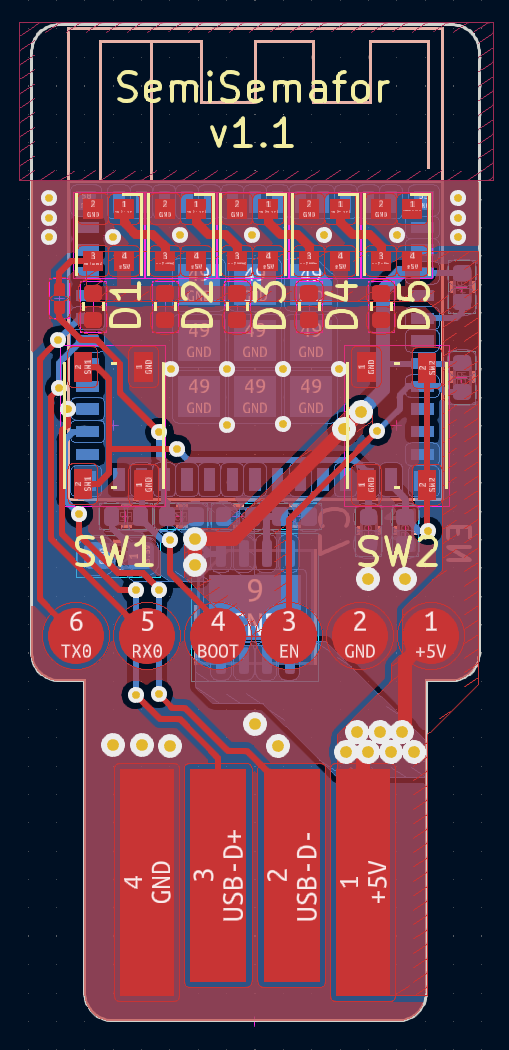
\includegraphics[width=\textwidth]{text/PraktickaCast/img/SemiSemafor-PCB.png}
%         \caption{Vzhled desky plošných spojů}
%         \label{fig:3D}
%     \end{minipage}
% \end{figure}

\chapter{Návrh statického zařízení}
% Celé zařízení je rozděleno na základní jednotku a~případné moduly, které zajistí nové herní možnosti.
% Například může jít o~připojení úložného prostoru nebo zvukového modulu, který poskytne jak plnohodnotný zvukový výstup tak vstup.

% \subsection{uživatelské požadavky}
Uživatelským požadavkem je statické zařízení sloužící jako herní stanoviště.
Vyžaduje tedy mobilitu jen v~rámci transportu na místo hry a~zpět, nikoliv v~rámci samotné hry.
Z~toho plynou požadavky na velikost výsledného zařízení.

Zařízení bude mít dva světelné kruhy složené z~60 inteligentních RGB LED.
Číslo 60 jsem zvolil, protože se jedná o~dostatečně jemné dělení, aby se daly dělat plynulé efekty.
Zároveň jde o~číslo, které koresponduje s~hodinovým ciferníkem a stupnicí na kompasu.
Jeden z~kruhů bude radiální a~druhý axiální.
Axiální je na horní straně zařízení a~slouží primárně jako odezva pro hráče na malou vzdálenost, např. při zadávání hesla.
Radiální kruh je pak také v~horní části zařízení a~slouží naopak pro signalizaci na delší vzdálenost, takový maják.

%TODO: dopsat a vygenerovat ilustraci
Uvnitř axiálního světelného kruhu se bude nacházet tzv. tlaková plocha.
\label{popisTlakovky} Jedná se o~ovládací prvek podobný dotykové ploše, s~tím rozdílem, že je schopen měřit i~sílu, která na něj působí.
Tento prvek je založen na měření rezonanční frekvence snímacích LC článků, nad kterými se nachází tlaková plocha.
Tlaková plocha je vodivý objekt, ve kterém se cívkou LC článku indukují vířivé proudy a následně se jimi indukují proudy zpět v cívce LC článku.
Tím plocha ovlivňuje indukčnost cívky a tedy i rezonanční frekvenci LC článku.
Ovlivnění indukčnosti je závislé na vzdálenosti plochy od cívky a tedy i na síle, která na plochu působí.
Velikost síly, která na plochu působí, totiž ovlivňuje její průhyb a tedy i vzdálenost od cívky.
Díky velkému rozlišení použitého čipu LDC1614 \cite{LDC1614} (28 bitů) je možné měřit změny vzdálenosti v řádu jednotek mikrometrů \cite{LDC1614LinearPositionSensing}.
Tato metoda je tedy schopna měřit vzdálenost plochy od jednotlivých cívek, ty jsou čtyři, a plochu tak snímají na čtyřech místech.
Následně je z těchto hodnot možno dopočítat, jak je plocha nakloněna a tím určit, kde se jí uživatel dotýká.
% Protože je zároveň možné určit i sílu jakou uživatel při dotyku vyvinul, dostal tento systém jméno tlaková plocha. % silová by bývalo přesnější ale nějak mi to nejde přes pysky

Aby bylo stanoviště reálně použitelné při hře, musí celou hru vydržet na baterii.
Není ojedinělé, aby měla outdoorová hra čtyři až pět hodin bez přestávky.
Plus je nutná časová rezerva a~čas na nastavování.
Čas, který zařízení zvládne běžet z~baterie, silně závisí na činnosti, ale nebylo by zrovna ideální, kdyby byla baterka, výrazně omezujícím faktorem.
Výdrž na jedno nabití by tedy měla být alespoň pět hodin.

Vzhledem k~plánu připojovat moduly je nutné navrhnout mechanizmus připojení.
Bylo by ideální, kdyby si mohl uživatel říct co bude hrát za hru a~podle toho si sám připojil moduly, které potřebuje.
Tomuto určitě nechci bránit, ale přímo to podporovat nese řadu problémů, jak ze strany konektoru a~mechaniky, tak ze strany softwaru.
Konektor by totiž musel být ideálně beznástrojově rozpojitelný a~opětovně spojitelný a~přitom dostatečně pevný, aby se zařízení mechanicky chovalo jako jeden celek.
Takový konektor je ale poměrně složité udělat, tak aby byl spolehlivý, a~tak jde v~tuto chvíli jen o možnost dalšího vývoje.
Ze softwarového pohledu jde pak o~problém jak detekovat konkrétní modul a~hlavně o~otázku jak se chovat k~modulům, které jsou potenciálně záměnné.
Dejme tomu, že máme modul klávesnici a~modul dvířka.
Dvířka jsou původně navržena primárně jako úložný prostor, díky detekci zavření je lze ale použít i~jako velmi pohodlná tlačítka a~v~některých hrách se proto používají jen jako tlačítka.
Potenciální modul klávesnice je ovšem jen suma tlačítek.
Při vytváření konkrétní hry na míru modulům, které herní návrhář má zrovna k~dispozici, je tento problém nepodstatný, protože sám návrhář rozhodne, co má jak být.
Ale ve chvíli, kdy jde o~hru navrženou pro jinou kombinaci modulů, nastává problém jak rozhodnout, zda se dají dvířka použít místo klávesnice nebo ne.
Abych se všem těmto problémům alespoň prozatím vyhnul, rozhodl jsme se, že doplnění či výměna modulu, půjde jen při servisním zásahu.
Problém záměny modulů pak budu řešit tím, že každá hra bude vytvořena jen pro konkrétní sadu modulů.

Některé hry vyžadují tak velké herní území, že by na komunikaci mezi stanovištěmi už nestačila WiFi ani Bluetooth, které AHS jinak využívá ke komunikaci (viz: \ref{sec:TypVzdaleneKomunikace}).
Proto bude mít AHS možnost připojení k~mobilní síti a~tedy připojení k~internetu (výběr viz: \ref{sec:TypVzdaleneKomunikace}).
Tím se rozšíří dosah AHS všude, kde je mobilní pokrytí a~také přibude další metoda jak se stanovištěm komunikovat.
V~rámci tohoto komunikačního modulu bude možné používat navíc i~GNSS \footnote{Global Navigation Satellite System}.
Vzhledem k~faktu, že se přece jen nejedná o~systém, který by využila většina her a~zároveň je poměrně drahý, došel jsem k~rozhodnutí mít jej jen jako doplnitelný modul.
Protože se ale jedná o~modul, který zprostředkovává komunikaci se světem, je pravděpodobné, že bude potřebovat převádět výrazně větší množství dat než běžný modul.
Primárně z~tohoto důvodu je tento modul připojen na samostatném konektoru, přímo uvnitř základního zařízení.
Potřebné antény budou už v~základním zařízení, ale samotný modul spadá do doplňkové výbavy.

V~řadě případů je užitečné mít možnost zvukové zpětné vazby.
Ideální by bylo moci přehrávat libovolnou nahrávku, většinou ale stačí jednoduchý tón, řekněme jako potvrzení zadaného hesla.
Možnost přehrávat plnohodnotnou nahrávku proto odsouvám na samostatný modul a~v základní jednotce pro jednoduchost postačí piezoměnič.

Z~požadavků mi vyplynulo zařízení, jehož vzhled je nastíněn na obrázku \ref{fig:AHS-nacrt}.
\begin{figure}
    \centering
    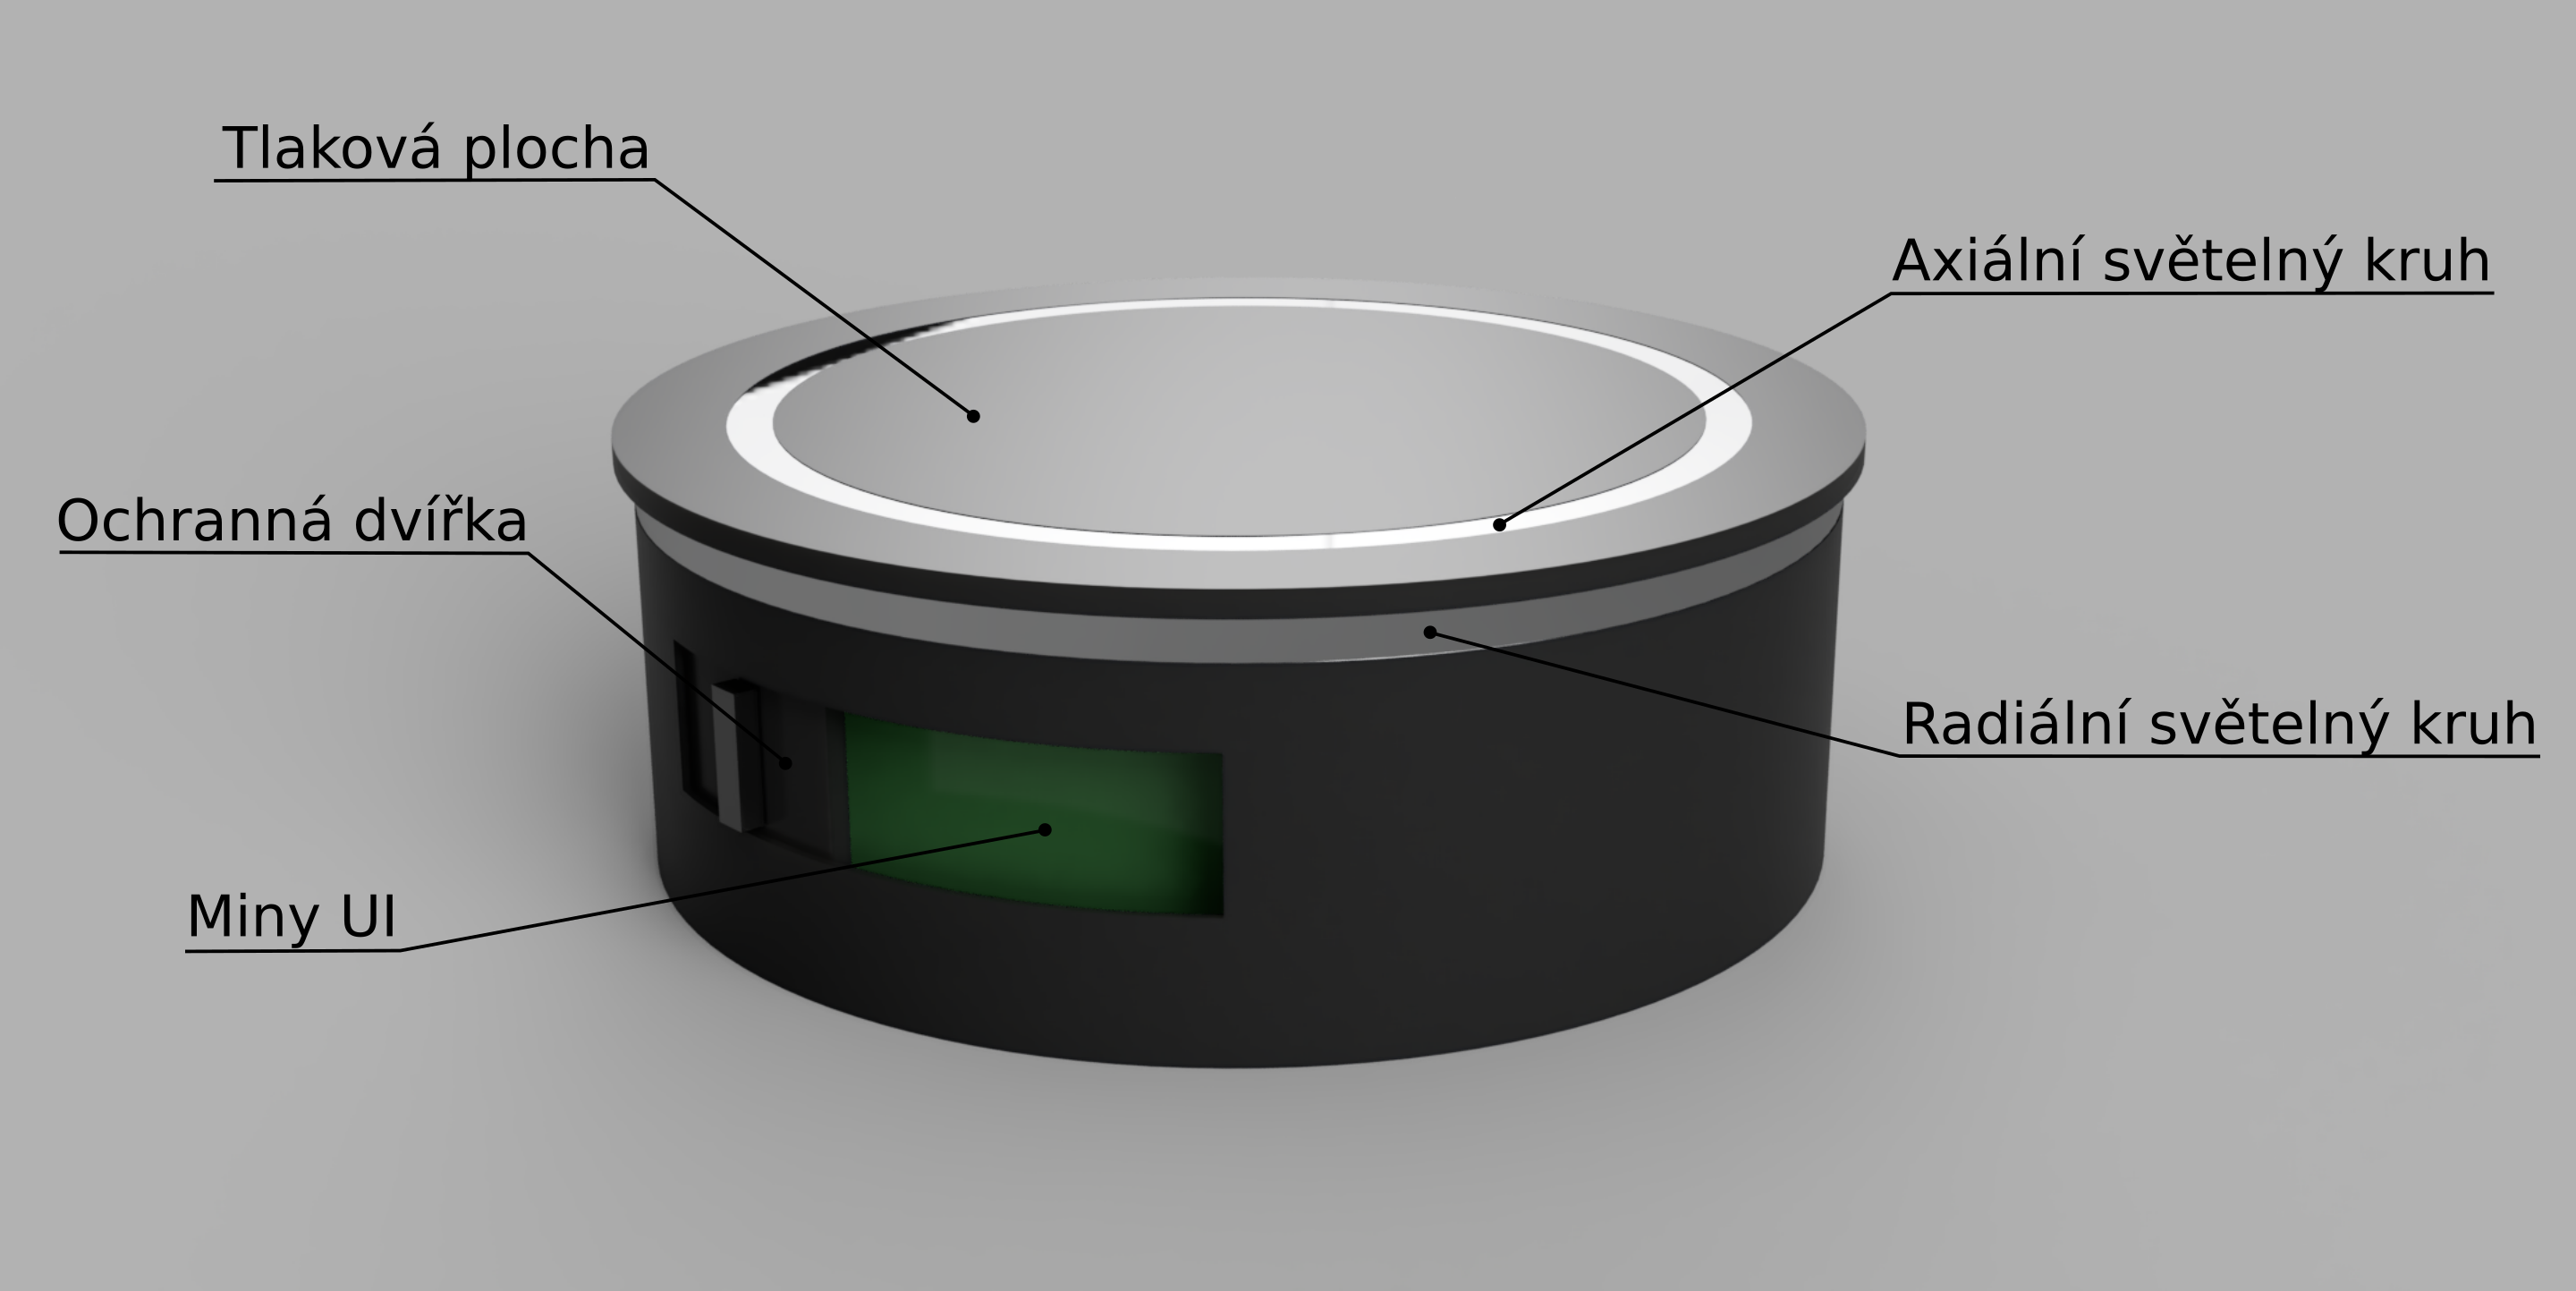
\includegraphics[width=\textwidth]{text/PraktickaCast/img/AHS-nacrt.png}
    \caption{Návrh vzhledu zařízení}
    \label{fig:AHS-nacrt}
\end{figure}

\newpage
\section{Struktura elektroniky základní jednotky}

Elektronika je rozdělena na tři samostatné PCB.
Jde o~hlavní desku, na které je většina elektroniky, o~desku s~hlavním uživatelským rozhraním (LED deska) a~o~obslužnou desku s~minimalistickým uživatelským rozhraním pro neherní obsluhu (Mini~UI).

\subsection{LED deska}
Na LED desce se nacházejí oba světelné kruhy a~elektronika pro snímání tlakové plochy, tedy LDC1614 \cite{LDC1614} a~jeho snímací LC články.
Právě snímaní tlakové plochy je jeden z~podstatných důvodů oddělení této elektroniky na samostatnou desku, zabere totiž docela dost prostoru.

\begin{itemize}
    \item Axiální LED kruh z~60 RGB LED WS2812
    \item Radiální LED kruh z~60 RGB LED WS2812
    \item LDC1614 nebo LDC1314 se čtyřmi snímacími LC články pro snímání tlakové plochy
    \item konektor na propojení s~hlavní deskou
\end{itemize}

\subsection{Mini UI}
Kvůli aktuální představě mechanické konstrukce není úplně dobře možné mít toto minimalistické uživatelské rozhraní na hlavní desce.
Proto jsem se rozhodl jej oddělit na samostatnou desku, na které bude jen pár tlačítek a~dvě signalizační LEDky.

\begin{itemize}
    \item RESET tlačítka
    \item BOOT tlačítka
    \item zapínací tlačítko
    \item dvě uživatelská tlačítka 
    \item dvě uživatelské LEDky
\end{itemize}

\subsection{Hlavní deska}
Na hlavní desce je většina systému základního zařízení.

Řídící mikrokontroler AHS je ESP32-S3 (výběr viz \ref{subs:vyberMikrokontroleru}).

Zdroj AHS je tvořen dvěma LiIon články 18650 v~paralelním uspořádání.
Paralelní uspořádání jsem zvolil tak, aby nebylo nutné řešit balancování článků.

Aby nebylo možné softwarově baterii podvybít, má AHS ochranu podvybitím, která celé zařízení vypne v~případě, že dojde k~vybití baterie pod 2.8V.
Pochopitelně software by měl vybitou baterii zaznamenat mnohem dřív a~chovat se podle toho, např. neumožnit spustit hru s~baterií při napětí 3.0V.

Na hlavní desce je i~nabíjecí elektronika.
Navíc, aby se minimalizoval čas nabíjení, zařízení podporuje standard Power Delivery a~to až do napětí 21V.

Protože různé periferie vyžadují různá napájecí a~komunikační napětí, je na hlavní desce hned pět napájecích větví.
\begin{itemize}
    \item VCC, napětí baterie sloužící jako zdroj pro ostatní napájecí větve a~pro napájení komunikačního modulu. 
    \item Napětí \(3.3\-[V]\) na napájení logické části celého základního zařízení.
    \item Napětí \(5.0\-[V]\) pro LED desku a~externí moduly
    \item Napětí \(1.8\-[V]\) pro napájení napěťových převodníků sloužících na komunikaci s~komunikačním modulem 
    \item V-USB, napětí \(5\- - \-21\-[V]\) z~USB-C konektoru pro nabíjení a~programování
\end{itemize}
Napětí větví \(3.3\-[V]\) a~\(1.8\-[V]\) je tvořeno pomocí LDO.
Na vytvoření větve \(5\-[V]\) je ale potřeba spínaný zdroj a~to primárně ze dvou důvodů.
Za prvé protože napětí baterie, ze které se tato větev napájí, má nižší napětí a~je jej tedy třeba vyspínat na napětí vyšší.
Za druhé tento zdroj poskytuje do systému mnohem větší proudy než druhé dvě větve a~bylo by tedy vhodné použít spínaný zdroj i~v případě použití sériového řazení článků.

\newpage
Na hlavní desce je také řada konektorů sloužící pro připojení ostatních systémů.
Jde o~konektory na:
\begin{itemize}
    \item propojení s~LED deskou                                            % samostatný objekt
    \item připojení Mini UI                                                 % samostatný objekt
    \item komunikační modul (M2 Konektor umožňuje použít různé moduly)      % externě definovaný objekt
    \item externí moduly                                                    % samostatný objekt
    \item USB-C (nabíjení a~programování AHS)                               % externě definovaný objekt
    \item programátor                                                       % samostatný objekt
\end{itemize}
Do konektorů by se dal zařadit i~držák na dva LiIon články 18650.

Jako jednoduchý zvukový výstup je na desce také piezoměnič.

\subsection{Výběr mikrokontroleru \label{subs:vyberMikrokontroleru}}
Požadavky na mikrokontroler jsou:
\begin{itemize}
    \item WiFi
    \item Bluetooth
    \item alespoň 3~UARTy
    \item alespoň 30 GPIO pinů
    \item I2C
    \item dostatečný výpočetní výkon pro hladký chod interpretru JavaScriptu nebo Pythonu
\end{itemize}

Dostupné možnosti jsou:
% \begin{itemize}
%     \item ESP32                 \cite{ESP32}
%     \item ESP32-S3              \cite{ESP32S3}
%     \item ESP32-C6              \cite{ESP32C6}
%     \item PIC32MZ-W1            \cite{PIC32MZ}
% \end{itemize}
\begin{figure}[h]
    \hspace{-20mm}
    \small
    \begin{tabular}{|l|l|l|l|l|c|}
        \hline
        Mikrokontroler              & Procesor      & Počet GPIO pinů    & Počet UARTů   & Počet I2C & Wi-Fi a Bluetooth                \\ \hline
        ESP32      \cite{ESP32}     & 2x Xtensa LX6 & 34                 & 3             & 2         & \textcolor{green}{\checkmark}    \\ \hline
        ESP32-S3   \cite{ESP32S3}   & 2x Xtensa LX7 & 45                 & 3             & 2         & \textcolor{green}{\checkmark}    \\ \hline
        ESP32-C6   \cite{ESP32C6}   & 1x RISC-V     & 34                 & 3             & 2         & \textcolor{green}{\checkmark}    \\ \hline
        PIC32MZ-W1 \cite{PIC32MZ}   & DS60001192    & 62                 & 3             & 2         & \textcolor{green}{\checkmark}    \\ \hline
    \end{tabular}
    \caption{Dostupné vyhovující mikrokontrolery}
    \label{tab:vyberMikrokontroleru}
\end{figure}
Při procházení stránek výrobců jsem nenašel jiný mikrokontroler, který by splňoval všechny požadavky \cite{NordicWiFi}.
Většina mikrokontrolerů s~integrovaným bezdrátovým rozhraním nemá WiFi a~Bluetooth dohromady, a~ty, co mají, mají zase nedostatek GPIO pinů.
Například nRF7000 \cite{nRF7000} má pouze 13 GPIO pinů, RTL8710 má 17 GPIO pinů \cite{RTL8710}, RTL8721 \cite{RTL8721DM} má GPIO pinů také 17. 
STM32WB55 \cite{STM32WB55} nebo MSP430BT5190 \cite{MSP430BT5190} zase nemají Wi-Fi.

% ESP32:
% \begin{itemize}
%     \item Procesor: Tensilica Xtensa LX6, 2~jádra, až \(240\-[MHz]\) \cite{ESP32}
%     \item Počet GPIO pinů: 34
%     \item Počet UARTů: 3
%     \item Počet I2C: 2
% \end{itemize}

ESP32 by bylo použito na modulu ESP32-wrover \cite{ESP32-WROOM}, který řeší anténu a flash~paměť.
Počet GPIO pinů mu tak klesne na 32, z čehož je 6 pinů připojeno na flash~paměť a jejich použití by tak bylo problematické, mikrokontroler proto z výběru vyřazuji.

% ESP32-C6:
% \begin{itemize}
%     \item Procesor: Tensilica Xtensa LX6, 1~jádro, až \(160\-[MHz]\) \cite{ESP32C6}
%     \item Počet GPIO pinů: 34
%     \item Počet UARTů: 3
%     \item Počet I2C: 2
% \end{itemize}

Stejně jako ESP32 by i ESP32-C6 bylo použito na modulu ESP32C6-WROOM \cite{ESP32C6-WROOM}, který řeší anténu a flash~paměť.
Počet GPIO pinů mu tak klesne na 23, mikrokontroler proto z výběru vyřazuji.

% ESP32-S3:
% \begin{itemize}
%     \item Procesor: Tensilica Xtensa LX7, 2~jádra, až \(240\-[MHz]\) \cite{ESP32S3}
%     \item Počet GPIO pinů: 45
%     \item Počet UARTů: 3
%     \item Počet I2C: 2
% \end{itemize}

I ESP32-S3 by bylo použito na modulu ESP32-S3-WROOM \cite{ESP32S3-WROOM}, který řeší anténu a flash~paměť.
Počet GPIO pinů mu tak klesne na 36, což je pořád dostatečné množství.

% PIC32MZ-W1:
% \begin{itemize}
%     \item Procesor: DS60001192, 1~jádro, až \(200\-[MHz]\) \cite{PIC32MZ}
%     \item Počet GPIO pinů: 62
%     \item Počet UARTů: 3
%     \item Počet I2C: 2
% \end{itemize}

PIC32MZ-W1 by bylo použito na modulu WFI32E01PC \cite{WFI32E01PC}, který řeší anténu a flash~paměť.
Počet GPIO pinů mu tak klesne na 37, což je pořád dostatečné množství.

\begin{figure}[h]
    \centering
    \begin{tabular}{|l|l|l|l|l|}
        \hline
        Mikrokontroler                  & Počet GPIO pinů    & vyhovuje?                     \\ \hline
        ESP32-WROOM     \cite{ESP32}    & 26                 & \textcolor{red}{$\times$}     \\ \hline
        ESP32-S3-WROOM  \cite{ESP32S3}  & 36                 & \textcolor{green}{\checkmark} \\ \hline
        ESP32-C6-WROOM  \cite{ESP32C6}  & 23                 & \textcolor{red}{$\times$}     \\ \hline
        WFI32E01PC      \cite{PIC32MZ}  & 37                 & \textcolor{green}{\checkmark} \\ \hline
    \end{tabular}
    \caption{Moduly s mikrokontrolery}
    \label{tab:ModulySMikrokontrolery}
\end{figure}

Jedním z požadavků na zařízení je dostatečný výpočetní výkon pro hladký chod interpretru JavaScriptu nebo Pythonu.
Výpočetní výkon se porovnává poněkud složitěji, protože se nejedná tak úplně o~jeden parametr.
V tomto případě je ale vhodné prozkoumat i dostupnost interpretru pro daný mikrokontroler.
Pro ESP32-S3 je dostupný JavaScriptový interpreter Jaculus \cite{Jaculus} i~interpretr jazyka Python MicroPython \cite{MicroPythonESP32S3}.
Pro PIC32MZ-W1 je dostupný interpreter jazyka Python MicroPython \cite{MicroPythonPIC32MZ-W1}, interpretter JavaScriptu jsem nenašel.
ESP32-S3 mi tak poskytuje výhodu v možnosti volby skriptovacího jazyka.

Další výhodou ESP32-S3 je jeho cena, která se pohybuje okolo \(4\-\$\) \cite{JSC-ESP32-S3}.
PIC32MZ-W1 je u JLCPCB za \(13.65\-\$\) \cite{JSC-WFI32}.
Navíc u JLCPCB je PIC32MZ-W1 sice v nabídce, ale není na skladě \cite{JSC-WFI32}, zatímco u ESP32-S3 je aktuálně dostupných 19 variant \cite{JSC-ESP32-S3}.

V mém případě má ESP32-S3 ještě jednu podstatnou výhodu, a tou je fakt, že s rodinou mikrokontrolerů ESP32 mám dlouholeté zkušenosti.
Z těchto důvodu jsem se rozhodl pro ESP32-S3.

\subsection{Propojení hlavní desky a~LED desky}
Mezi hlavní deskou a~LED deskou je třeba převést napájení a~několik signálů.
LED deska vyžaduje na konektoru přítomnost dvou napájecích větví \(5\-[V]\) pro světelné kruhy a~\(3.3\-[v]\) pro snímání tlakové plochy.
Protože do LEDek může téct proud až 5A a~může být zároveň i~docela rychle spínaný, považuji za rozumné oddělit napájecím větvím zem.
Oddělení je tedy provedeno už na konektoru hlavní desky.

Na samotné propojení jsem se rozhodl použít FFC kabel s~roztečí \(0.5\-[mm]\).
Jedním vodičem takovéhoto kabelu lze vést proud maximálně \(0.4\-[A]\) \cite{FFC-konektor}.
Protože ale potřebuji dodat proud až 5A, použiji 13 vodičů vedle sebe jakožto nejmenší počet, který přenese požadovaný proud v~rámci daných mezí.

Mimo napájení je tímto propojením veden i~signál s~daty pro světelné kruhy a~I2C sběrnice s~interruptem pro připojení čipu LDC1614 \cite{LDC1614}.

Vzhledem k~počtu potřebných vodičů (konkrétně 32) jsem se rozhodl použít běžný FFC konektor se 40 kontakty s~tím, že zbylé kontakty se mohou hodit v~budoucnu.

\subsection{Modulový konektor \label{sec:ModulovyKonektor}}
Modulovým konektorem je vedeno \(5\-[V]\) jako napájení pro moduly a~UART s~interruptem pro komunikaci.
Nad volbou komunikační sběrnice jsem strávil poměrně dost času přemýšlením.
Původně jsem uvažoval o~využití RS485 jakožto odolné sběrnice, u~které by v~případě potřeby nemusel být problém ani delší kabel.
RS485 má ale nevýhodu v~tom, že potřebuje dodatečný hardware, kterému bych se hlavně na modulech rád vyhnul.
Stejný problém nastal u~CANu a~USB, které by navíc mělo výhodu kompatibility s~velkým množstvím hotových zařízení.

V~první úvaze o~UARTu jsem jej nejprve zavrhl kvůli potenciální náročnosti na přeposílání dat mezi moduly.
Při standardním použití bych totiž moduly řadil za sebe.
Prvnímu modulu by tak chodili data pro všechny ostatní moduly a~musel by je přeposílat dál, což by mohlo stát nezanedbatelné množství procesorového času.
V~jisté chvíli jsem ale narazil na nestandardní komunikaci pomocí UARTu implementované v~projektu Servio \cite{Servio}.
Tato implementace používá UART jako sběrnici.
Namísto standardního použití pro komunikace jeden s~jedním tak může komunikovat jeden s~více.
Na tomto řešení je výhodné, že nevyžaduje žádný dodatečný hardware a~prakticky každý dnešní mikrokontroler je možné k~této sběrnici velmi snadno připojit.
Ve srovnání s~RS485 je sice mnohem méně odolná proti rušení, ale uvnitř zařízení nebude linka vedena na víc než malé desítky centimetrů.
Komunikace na delším kabelu je pak jednoduše nahraditelná bezdrátovou komunikací a~není tak potřebné, aby to nativně umožňovala tato sběrnice.
Každopádně v~případě potřeby delšího kabelu je možné navrhnout externí modul, který s~této sběrnice velmi jednoduše udělá RS485 pro externí využití.
Alternativně by se pro komunikaci na delším kabelu dalo použít USB, které je společně s~nabíjením přivedeno na USB-C.

Všechny moduly jsou tedy připojeny na jeden RX pin AHS.
Proto musí firmware AHS zajistit, aby dva moduly nevysílaly současně.
Aby se zabránilo možným zkratům, jako ochranu má každý modul své piny UARTu připojeny přes rezistor \(180\-[\Omega]\).
Interrupt pin modulů se naopak chová jako open-collector a~na straně hlavního zařízení je na něj tedy připojen pull-up rezistor.
Abych alespoň trochu zvýšil odolnost linky proti rušení, přidám na přijímací stranu pull-up rezistor.
Cílem je zvýšení komunikačního proudu, aby se případný proud vyvolaný rušením neprojevil.
V~neposlední řadě mají všechny piny na konektoru ESD ochranu.

\newpage
\subsection{Konektor programátor}
Zařízení se dá jednoduše programovat přes USB-C, tento kanál se ale dá softwarově narušit a~pro takové případy je tu konektor na programátor.
Jde o~šest plošek, na které se programátor připojuje pomocí pogo-pinů.
Programátor sice obsahuje jen jednoduchou elektroniku, která by mohla být i~přímo v~elektronice AHS, ale ve většině případů by byla zbytečná.
Ve chvíli, kdy by byla potřeba, je stejně nutná odborná obsluha a~pro tu není problém použít programátor.

\begin{figure}[h]
    \vspace{-3mm}
    \centering
    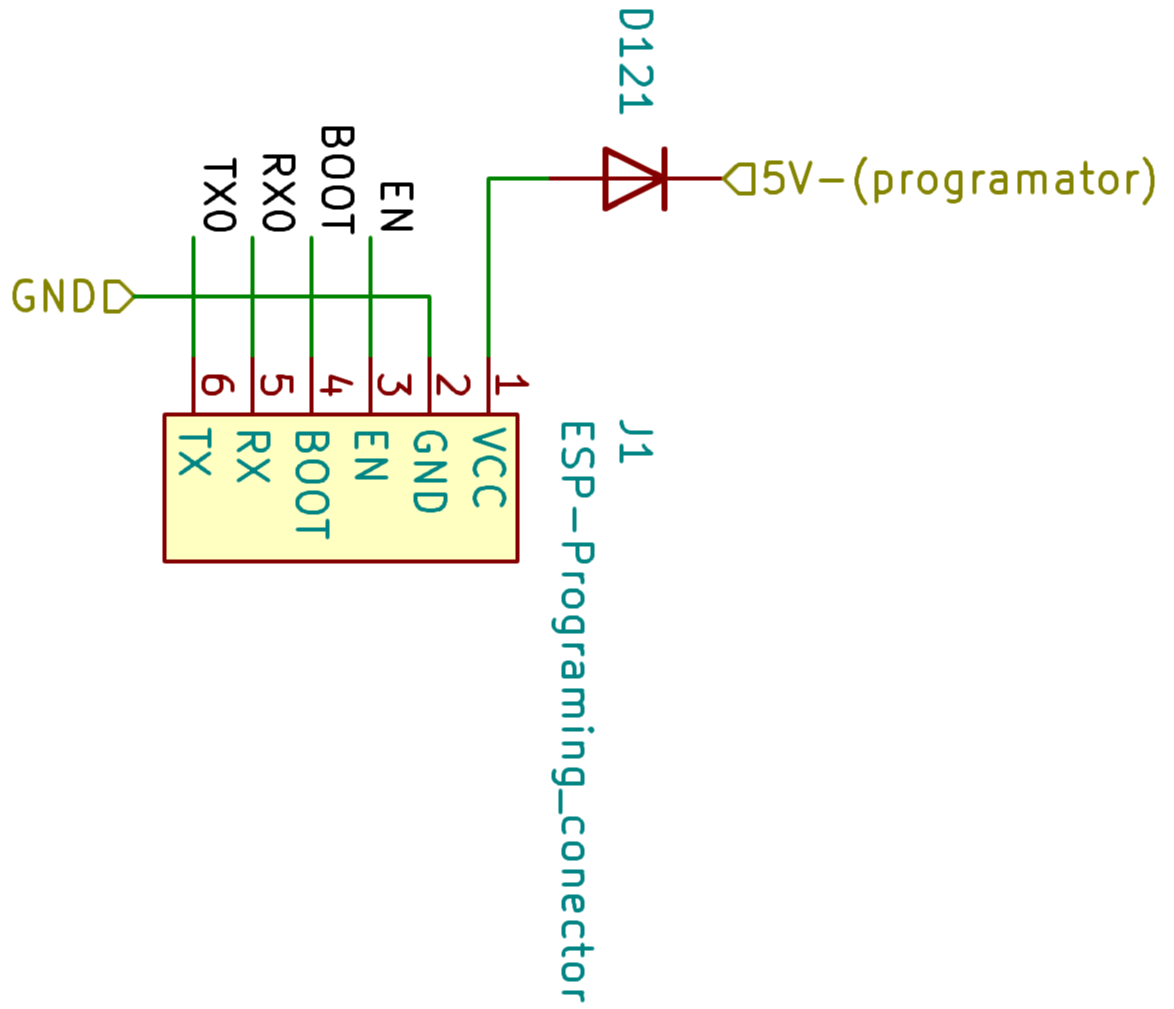
\includegraphics[width=\textwidth]{text/TeoretickyUvod/AplikaceHernichZarizeni/img/programator.png}
    \caption{Programovací konektor}
    \label{fig:programator}
\end{figure}
Aby bylo možné zařízení programovat přes dedikovaný programovací konektor, je na konektoru i~\(5\-[V]\) napájení.
To ale způsobuje problém ve chvíli, kdy je zařízení zároveň připojeno přes USB-C, protože se v~tu chvíli tyto zdroje zkratují.
% Proto je na konektoru programátor i~ochrana, která v~případě připojení USB-C odpojí napájení z~programátoru, neboli jedna dioda. %jako vtip který vymyslel gitkopilot super 
Proto je toto napájení přivedeno přes diodu, která v~případě připojení USB-C odpojí napájení z~programátoru.
Zapojení konektoru je vidět na obrázku \ref{fig:programator}.

\subsection{USB-C}
Jako napájecí a~programovací konektor je použito USB-C.
Díky němu je možné podporovat standard Power Delivery využitý pro zrychlení nabíjení.
Konektor je ale použit i~na pohodlnější programování zařízení, bez potřeby programátoru.

\subsection{Konektor komunikačního modulu}
Pro připojení komunikačního modulu jsem zvolil konektor M2 typ-B jakožto standard pro tyto moduly.
Díky tomuto konektoru mohu jednoduše připojit různé LTE a~GNSS moduly.


%%% Vložení souboru 'text/zaver' se závěrem
\chapter*{Závěr}
\phantomsection
\addcontentsline{toc}{chapter}{Závěr}

Shrnutí studentské práce.


%%% Vložení souboru 'text/literatura' se seznamem zdrojů
% \section{Použité zdroje}
% \begin{refsection}
%     \nocite{*}
%     \printbibliography[type=online,title={Online články a dokumenty}]
%     \printbibliography[type=manual,title={Katalogové listy důležitých součástek}]
% \end{refsection}
\clearpage
\section{Použité zdroje}
\nocite{*}
\printbibliography[type=online,title={Online články a dokumenty}, heading=subbibliography]
\printbibliography[type=manual,title={Katalogové listy důležitých součástek}, heading=subbibliography]

%%% Vložení souboru 'text/zkratky' se seznam použitých symbolů, veličin a zkratek
\cleardoublepage
\chapter*{\listofabbrevname}
\phantomsection
\addcontentsline{toc}{chapter}{\listofabbrevname}

\begin{acronym}[KolikMista]

	\acro{zkTemp}		% název
		[Šířka levého sloupce Seznamu symbolů a zkratek]								% zkratka
		{je určena šířkou parametru prostředí \texttt{acronym} (viz řádek~1 výpisu zdrojáku na~str.\,\pageref{lst:zkratky})}
											% rozvinutí zkratky

	\acro{AHS}
		{Automatické Herní Stanoviště}

	\acro{LDO}		% název/zkratka
		{Low-dropout regulator - regulátor napětí s nízkým úbytkem}
											% rozvinutí zkratky
	%%% bsymfvz
	\acro{FFC}						% název
		[\ensuremath{f_\textind{vz}}] % symbol
		{Flexible flat cable - plochý ohební kabel}					% popis
	%%% esymfvz

\end{acronym}


%%% Začátek příloh
\appendix

%%% Vysázení seznamu příloh
% (vynechejte, pokud máte dvě nebo méně příloh)
\listofappendices

%%% Vložení souboru 'text/prilohy' s přílohami
% Obvykle je přítomen alespoň popis co najdeme na přiloženém médiu
% \chapter{Některé příkazy balíčku \texttt{thesis}}

\section{Příkazy pro sazbu veličin a jednotek}

\begin{table}[!h]
  \caption[Přehled příkazů]{Přehled příkazů pro matematické prostředí }
  \begin{center}
  	\small
	  \begin{tabular}{|c|c|c|c|}
	    \hline
	    Příkaz    						& Příklad 					& Zdroj příkladu  							& Význam  \\
	    \hline\hline
	    \verb|\textind{...}|	& $\beta_\textind{max}$ 	& \verb|$\beta_\textind{max}$|	& textový index \\
	    \hline
	    \verb|\const{...}| 		& $\const{U}_\textind{in}$ 				& \verb|$\const{U}_\textind{in}$|		& konstantní veličina \\
	    \hline
	    \verb|\var{...}| 		& $\var{u}_\textind{in}$ & \verb|$\var{u}_\textind{in}$| & proměnná veličina \\
	    \hline
	    \verb|\complex{...}| 	& $\complex{u}_\textind{in}$ & \verb|$\complex{u}_\textind{in}$| & komplexní veličina \\
	    \hline
	    \verb|\vect{...}| 		& $\vect{y}$ 						& \verb|$\vect{y}$| & vektor \\
	    \hline
	    \verb|\mat{...}| 	& $\mat{Z}$ 						& \verb|$\mat{Z}$| & matice \\
	    \hline
	    \verb|\unit{...}| 		& $\unit{kV}$ 						& \verb|$\unit{kV}$|\quad či\ \, \verb|\unit{kV}| & jednotka \\
	    \hline
	  \end{tabular}
  \end{center}
\end{table}



%\newpage
\section{Příkazy pro sazbu symbolů}

\begin{itemize}
  \item
    \verb|\E|, \verb|\eul| -- sazba Eulerova čísla: $\eul$,
  \item
    \verb|\J|, \verb|\jmag|, \verb|\I|, \verb|\imag| -- sazba imaginární jednotky: $\jmag$, $\imag$,
  \item
    \verb|\dif| -- sazba diferenciálu: $\dif$,
  \item
    \verb|\sinc| -- sazba funkce: $\sinc$,
  \item
    \verb|\mikro| -- sazba symbolu mikro stojatým písmem%
			\footnote{znak pochází z~balíčku \texttt{textcomp}}: $\mikro$,
	\item
		\verb|\uppi| -- sazba symbolu $\uppi$
			(stojaté řecké pí, na rozdíl od \verb|\pi|, což sází $\pi$).
\end{itemize}
%
Všechny symboly jsou určeny pro matematický mód, vyjma \verb|\mikro|, jenž je\\ použitelný rovněž v~textovém módu.
%$\upmikro$


\chapter{Druhá příloha}

\begin{figure}[!h]
  \begin{center}
    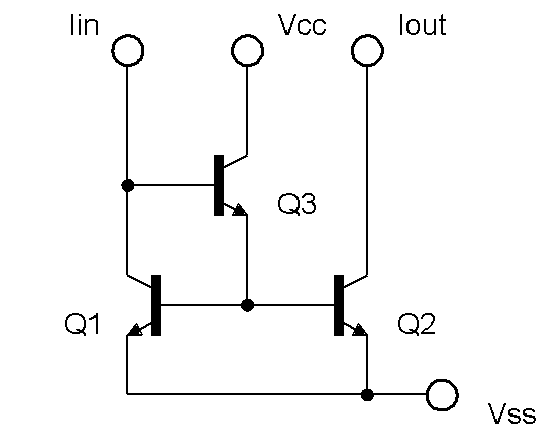
\includegraphics[scale=0.5]{obrazky/ZlepseneWilsonovoZrcadloNPN}
  \end{center}
  \caption[Alenčino zrcadlo]{Zlepšené Wilsonovo proudové zrcadlo.}
\end{figure}

Pro sazbu vektorových obrázků přímo v~\LaTeX{}u je možné doporučit balíček \href{https://www.ctan.org/pkg/pgf}{\texttt{TikZ}}.
Příklady sazby je možné najít na \href{http://www.texample.net/tikz/examples/}{\TeX{}ample}.
Pro vyzkoušení je možné použít programy QTikz nebo TikzEdt.




\chapter{Příklad sazby zdrojových kódů}

\section{Balíček \texttt{listings}}

Pro vysázení zdrojových souborů je možné použít balíček \href{https://www.ctan.org/pkg/listings}{\texttt{listings}}.
Balíček zavádí nové prostředí \texttt{lstlisting} pro sazbu zdrojových kódů, jako například:
%
\begin{lstlisting}[language={[LaTeX]TeX}]
\section{Balíček lstlistings}
Pro vysázení zdrojových souborů je možné použít
	balíček \href{https://www.ctan.org/pkg/listings}%
	{\texttt{listings}}.
Balíček zavádí nové prostředí \texttt{lstlisting} pro
	sazbu zdrojových kódů.
\end{lstlisting}
%
Podporuje množství programovacích jazyků.
Kód k~vysázení může být načítán přímo ze zdrojových souborů.
Umožňuje vkládat čísla řádků nebo vypisovat jen vybrané úseky kódu.
Např.:

\noindent
Zkratky jsou sázeny v~prostředí \texttt{acronym}:
\label{lst:zkratky}
\lstinputlisting[language={[LaTeX]TeX},nolol,numbers=left, firstnumber=6, firstline=6,lastline=6]{text/zkratky.tex}
%
Šířka textu volitelného parametru \verb|KolikMista| udává šířku prvního sloupce se zkratkami.
Proto by měla být zadávána nejdelší zkratka nebo symbol.
Příklad definice zkratky \acs{symfvz} je na výpisu \ref{lst:symfvz}.

\shorthandoff{-}
\lstinputlisting[language={[LaTeX]TeX},frame=single,caption={Ukázka sazby zkratek},label=lst:symfvz,numbers=left,linerange={bsymfvz-\%\%\%\ esymfvz},includerangemarker=false]{text/zkratky.tex}
\shorthandon{-}

\noindent
Ukončení seznamu je provedeno ukončením prostředí:
\lstinputlisting[language={[LaTeX]TeX},nolol,numbers=left,firstnumber=26,linerange=26]{text/zkratky.tex}

\vspace{\fill}

\noindent
{\bf Poznámka k~výpisům s~použitím volby jazyka \verb|czech| nebo \verb|slovak|:}\newline
Pokud Váš zdrojový kód obsahuje znak spojovníku \verb|-|, pak překlad může skončit chybou.
Ta je způsobená tím, že znak \verb|-| je v~českém nebo slovenském nastavení balíčku \verb|babel| tzv.\ aktivním znakem.
Přepněte znak \verb|-| na neaktivní příkazem \verb|\shorthandoff{-}| těsně před výpisem a hned za ním jej vraťte na aktivní příkazem \verb|\shorthandon{-}|.
Podobně jako to je ukázáno ve zdrojovém kódu šablony.


\clearpage

%\section{Výpis kódu prostředí Matlab}
Na výpisu \ref{lst:priklad.vypis.kodu.Matlab} naleznete příklad kódu pro Matlab, na výpisu \ref{lst:priklad.vypis.kodu.C} zase pro jazyk~C.

\lstnewenvironment{matlab}[1][]{%
\iflanguage{czech}{\shorthandoff{-}}{}%
\iflanguage{slovak}{\shorthandoff{-}}{}%
\lstset{language=Matlab,numbers=left,#1}%
}{%
\iflanguage{slovak}{\shorthandon{-}}{}%
\iflanguage{czech}{\shorthandon{-}}{}%
}

\begin{matlab}[frame=single,float=htbp,caption={Příklad Schur-Cohnova testu stability v~prostředí Matlab.},label=lst:priklad.vypis.kodu.Matlab,numberstyle=\scriptsize, numbersep=7pt]
%% Priklad testovani stability filtru

% koeficienty polynomu ve jmenovateli
a = [ 5, 11.2, 5.44, -0.384, -2.3552, -1.2288];
disp( 'Polynom:'); disp(poly2str( a, 'z'))

disp('Kontrola pomoci korenu polynomu:');
zx = roots( a);
if( all( abs( zx) < 1))
    disp('System je stabilni')
else
    disp('System je nestabilni nebo na mezi stability');
end

disp(' '); disp('Kontrola pomoci Schur-Cohn:');
ma = zeros( length(a)-1,length(a));
ma(1,:) = a/a(1);
for( k = 1:length(a)-2)
    aa = ma(k,1:end-k+1);
    bb = fliplr( aa);
    ma(k+1,1:end-k+1) = (aa-aa(end)*bb)/(1-aa(end)^2);
end

if( all( abs( diag( ma.'))))
    disp('System je stabilni')
else
    disp('System je nestabilni nebo na mezi stability');
end
\end{matlab}

\noindent
\begin{minipage}{\linewidth}


%\section{Výpis kódu jazyka C}

\begin{lstlisting}[frame=single,numbers=right,caption={Příklad implementace první kanonické formy v~jazyce C.},label=lst:priklad.vypis.kodu.C,basicstyle=\ttfamily\small, keywordstyle=\color{black}\bfseries\underbar,]
// první kanonická forma
short fxdf2t( short coef[][5], short sample)
{
	static int v1[SECTIONS] = {0,0},v2[SECTIONS] = {0,0};
	int x, y, accu;
	short k;

	x = sample;
	for( k = 0; k < SECTIONS; k++){
		accu = v1[k] >> 1;
		y = _sadd( accu, _smpy( coef[k][0], x));
		y = _sshl(y, 1) >> 16;

		accu = v2[k] >> 1;
		accu = _sadd( accu, _smpy( coef[k][1], x));
		accu = _sadd( accu, _smpy( coef[k][2], y));
		v1[k] = _sshl( accu, 1);

		accu = _smpy( coef[k][3], x);
		accu = _sadd( accu, _smpy( coef[k][4], y));
		v2[k] = _sshl( accu, 1);

		x = y;
	}
	return( y);
}
\end{lstlisting}
\end{minipage}







\chapter{Obsah elektronické přílohy}
Elektronická příloha je často nedílnou součástí semestrální nebo závěrečné práce.
Vkládá se do informačního systému VUT v~Brně ve vhodném formátu (ZIP, PDF\,\dots).

Nezapomeňte uvést, co čtenář v~této příloze najde.
Je vhodné okomentovat obsah každého adresáře, specifikovat, který soubor obsahuje důležitá nastavení, který soubor je určen ke spuštění, uvést nastavení kompilátoru atd.
Také je dobře napsat, v~jaké verzi software byl kód testován (např.\ Matlab 2018b).
Pokud bylo cílem práce vytvořit hardwarové zařízení,
musí elektronická příloha obsahovat veškeré podklady pro výrobu (např.\ soubory s~návrhem DPS v~Eagle).

Pokud je souborů hodně a jsou organizovány ve více složkách, je možné pro výpis adresářové struktury použít balíček \href{https://www.ctan.org/pkg/dirtree}{\texttt{dirtree}}.

\bigskip

{\small
%
\dirtree{%.
.1 /\DTcomment{kořenový adresář přiloženého archivu}.
.2 logo\DTcomment{loga školy a fakulty}.
.3 BUT\_abbreviation\_color\_PANTONE\_EN.pdf.
.3 BUT\_color\_PANTONE\_EN.pdf.
.3 FEEC\_abbreviation\_color\_PANTONE\_EN.pdf.
.3 FEKT\_zkratka\_barevne\_PANTONE\_CZ.pdf.
.3 UTKO\_color\_PANTONE\_CZ.pdf.
.3 UTKO\_color\_PANTONE\_EN.pdf.
.3 VUT\_barevne\_PANTONE\_CZ.pdf.
.3 VUT\_symbol\_barevne\_PANTONE\_CZ.pdf.
.3 VUT\_zkratka\_barevne\_PANTONE\_CZ.pdf.
.2 obrazky\DTcomment{ostatní obrázky}.
.3 soucastky.png.
.3 spoje.png.
.3 ZlepseneWilsonovoZrcadloNPN.png.
.3 ZlepseneWilsonovoZrcadloPNP.png.
.2 pdf\DTcomment{pdf stránky generované informačním systémem}.
.3 student-desky.pdf.
.3 student-titulka.pdf.
.3 student-zadani.pdf.
.2 text\DTcomment{zdrojové textové soubory}.
.3 literatura.tex.
.3 prilohy.tex.
.3 reseni.tex.
.3 uvod.tex.
.3 vysledky.tex.
.3 zaver.tex.
.3 zkratky.tex.
%.2 navod-sablona\_FEKT.pdf\DTcomment{návod na používání šablony}.
.2 sablona-obhaj.tex\DTcomment{hlavní soubor pro sazbu prezentace k~obhajobě}.
%.2 readme.txt\DTcomment{soubor s~popisem obsahu CD}.
.2 sablona-prace.tex\DTcomment{hlavní soubor pro sazbu kvalifikační práce}.
.2 thesis.sty\DTcomment{balíček pro sazbu kvalifikačních prací}.
}
}


\end{document}